\documentclass[12pt,a4paper,oneside]{book} %TODO: Per stampare metti in twoside
\usepackage[italian]{babel}

\title{Analisi e sviluppo di middleware DDS per la gestione dei consumi in sistemi HPC}
\author{Giacomo Madella}
\date{Aprile 2021}


% setup.tex

% Codifica dei caratteri e lingua
\usepackage[T1]{fontenc}
\usepackage{newlfont}
\usepackage[italian]{babel}

% Margini e formattazione della pagina
\usepackage{geometry} %[a4paper, top=2.5cm, bottom=2.5cm, left=3cm, right=3cm, bindingoffset=0cm]

% \usepackage{amssymb}
% \usepackage{latexsym}
% \usepackage{mathtools}
\usepackage{mathptmx}

\usepackage[acronym,nopostdot]{glossaries} % Carica il pacchetto glossaries



\def\arraystretch{1.5}% tabular stretch

% Pacchetto per l'inclusione di immagini
\usepackage{graphicx}
\graphicspath{ {../img/} }
\usepackage{wrapfig}

% Pacchetto per la gestione delle unità di misura
\usepackage{siunitx}

% Pacchetto per l'impaginazione avanzata
\usepackage{fancyhdr}

% Pacchetto per la gestione avanzata delle tabelle
\usepackage{tabularx}

% Pacchetto per la creazione di liste personalizzate
\usepackage{enumitem}

\usepackage{graphicx} % utils per le immagini
\usepackage{float} % Per le immagini [H]
\usepackage{subcaption} % Per le immagini affiancate


% Pacchetto per la creazione di collegamenti ipertestuali
\usepackage{amsthm}
\usepackage{hyperref}
\hypersetup{
    colorlinks=true,
    linkcolor=black,
    citecolor=cyan,
    filecolor=magenta,
    urlcolor=cyan,
}
\usepackage{cleveref}

%\usepackage{indentfirst}%%libreria per avere l'indentazione all'inizio dei capitoli, ...


% Pacchetto per la formattazione avanzata delle didascalie delle figure e delle tabelle
\usepackage[font=small, labelfont=bf, labelsep=period]{caption}

% Pacchetto per l'uso di colori
\usepackage{xcolor}

% Pacchetto per la formattazione avanzata delle pagine dei titoli dei capitoli
\usepackage{titlesec}

% Pacchetto per la creazione di elenchi puntati personalizzati
\usepackage{enumitem}

% Altri pacchetti personalizzati e configurazioni possono essere aggiunti qui

% Configurazioni personalizzate
% Esempio: Cambia il formato dei titoli dei capitoli
%\titleformat{\chapter}[display]{\normalfont\huge\bfseries}{\chaptertitlename\ \thechapter}{20pt}{\Huge}
\usepackage{afterpage}
\newcommand\blankpage{%
    \null%
    \thispagestyle{empty}%
    %\addtocounter{page}{-1}%
    \newpage}
\usepackage[sorting=none]{biblatex}
\usepackage{csquotes}
\addbibresource{setup/references.bib}

% Fine del file setup.tex

% Old files
% \usepackage[colorinlistoftodos]{todonotes}
% %\usepackage{ulem}
% \usepackage{graphicx}%libreria per inserire grafici
% \graphicspath{ {../img/} }
% %%librerie matematiche


% \usepackage{hyperref}
% \hypersetup{
%     colorlinks=false,
%     linkcolor=blue,
%     filecolor=magenta,      
%     urlcolor=cyan,
% }
% \usepackage{fancyhdr} %%libreria per impostare il documento


% \usepackage{cleveref}

% \usepackage{listings}
% \usepackage{booktabs}
% \usepackage{subfig}
% \usepackage{float}

% \usepackage{multicol}

% \usepackage{adjustbox}


% \usepackage{vmargin} 
% \oddsidemargin=30pt \evensidemargin=20pt%impostano i margini
% \hyphenation{sil-la-ba-zio-ne pa-ren-te-si}%serve per la 
% \hypersetup{
%     colorlinks,
%     citecolor=black,
%     filecolor=black,
%     linkcolor=black,
%     urlcolor=black
% }
% \usepackage{enumerate}% http://ctan.org/pkg/enumerate
% \lstloadlanguages{bash}%\titleformat{\chapter}[hang]{\Huge\bfseries}{\thechapter\hsp\textcolor{gray75}{|}\hsp}{0pt}{\Huge\bfseries}
% %\lstinputlisting{NOME_FILE.ESTENSIONE} inserire direttamente il file
% %Dloating Figures
% \usepackage{wrapfig}

% %\geometry{bottom=3cm}
% %Times new roman

% %Interlinea
%  \linespread{1.3}                        %comando per impostare l'interlinea

% \renewcommand{\baselinestretch}{1.3} 


% % For images---------------------------------------

% % If you use the hyperref package, please uncomment the following line
% % to display URLs in blue roman font according to Springer's eBook style:
% %\renewcommand\UrlFont{\color{blue}\rmfamily}

% % New commands
% %\newcommand{\NDA}[1]{\todo[inline,color=cyan]{\textit{[Andrea: #1]}}}
% %\newcommand{\NDM}[1]{\todo[inline,color=red]{\textit{[Martin: #2]}}}

% % \hyphenation{com-pu-ta-tion-ally com-pu-ta-ti-on-ally-in-ten-si-ve}

\makenoidxglossaries

\newglossaryentry{Real-Time}{
  name={Real-Time},
  description={In tempo reale, con latenze molto basse},
  sort={Real-Time}
}
\newglossaryentry{Bash}{
  name={Bash},
  description={Bourne Angain Shell, linguaggio di scripting},
  sort={Bash}
}

\newglossaryentry{Ntpd}{
  name={ntpd},
  description={},
  sort={}
}

\newglossaryentry{x86}{
  name={},
  description={},
  sort={}
}

\newglossaryentry{Kernel}{
  name={kernel},
  description={},
  sort={}
}

\newglossaryentry{assembly}{
  name={assembly},
  description={},
  sort={}
}

\newglossaryentry{overhead}{
  name={overhead},
  description={},
  sort={}
}

\newglossaryentry{multicasting}{
  name={},
  description={},
  sort={}
}
\newglossaryentry{}{
  name={},
  description={},
  sort={}
}

\begin{document}  

%\setmarginsrb{3 cm}{2 cm}{3 cm}{0 cm}{-1 cm}{1 cm}{0 cm}{1.5 cm}
\thispagestyle{empty}%

\begin{titlepage}
	\begin{center}
		{{\Large{\textsc{Alma Mater Studiorum $\cdot$ Universit\`a di
		Bologna}}}} \rule[0.1cm]{14cm}{0.1mm}
		\rule[0.5cm]{14cm}{0.6mm}
			% \centering
			%\includegraphics[width=0.35\textwidth]{Immagini/Senza titolo-1.png}
			\large{\textsc{Corso di Laurea Magistrale in Ingegneria Informatica}}
			\\[1.8cm]
			\LARGE
			{\bfseries Analisi e sviluppo di middleware DDS per la gestione dei consumi in sistemi HPC}\\[1.2cm]
	\end{center}
	\vspace{4.5cm}
	\vfill
	\begin{minipage}{0.35\textwidth}
		{\bfseries Relatore}\\
		Prof. Andrea Bartolini 
	\end{minipage}
	\hfill
	\begin{minipage}{0.35\textwidth}
		\begin{flushright} {\bfseries Candidato}\\
		Giacomo Madella \end{flushright} 
	\end{minipage} \\
\begin{center}
	Ottobre 2023
\end{center}

\end{titlepage}



% %\title{A secure and distributed middleware for green computing} %
% \title{An interoperable runtime for distributed power management of large-scale HPC systems based on DDS.}
% % TITLE : sullo sviluppo di un run-time per il power management basato su DDS, astratto all’interno di una libreria simil ROS2
% \titlerunning{An interoperable runtime for green computing}
% \author{Giacomo Madella}
% \authorrunning{Madella}
% \institute{Alma Mater Studiorum, Università di Bologna \\
% Research Topic: Piattaforme distribuite, sicure e interoperabili per l'efficientamento dei sistemi di calcolo larga scala}
% \maketitle              % typeset the header of the contribution


\afterpage{\blankpage}

\thispagestyle{empty}%
\section*{Abstract}
\label{TODO}
Nei sistemi di High-Performance Computing (HPC), la gestione energetica è diventata una delle principali preoccupazioni, non solo a causa dei costi monetari, ma anche per la sostenibilità ambientale e per la progettazione di nuove generazioni di supercomputer\cite{growth}. Perpendicolarmente all'aumento della potenza computazionale richiesta, le tecnologie associate allo sviluppo dei componenti che stanno alla base dei processori, si sono avvicinati sempre più ai loro limiti fisici. E' nato con questo, il concetto di Power Management cercando di definire un modello software con il compito di gestire la potenza di sistemi di HPC. Data l'eterogeneità di questi sistemi, nel corso degli anni sono stati proposti sempre più strumenti in grado di funzionare su una specifica configurazione hardware e cercando di risolvere un sottoinsieme limitato di problemi. %Al giorno d'oggi ci sarebbe la necessità di un software unito, comune ed in grado di operare su diverse tipologie di architetture.
Lo scopo di questa tesi è di testare un middleware di comunicazione basato su Data Distribution Service(DDS), che faciliterebbe lo scambio di informazioni tra diversi software di Power Management. Questo permetterebbe di creare un Power Stack interoperable e con una visione di insieme. Successivamente sarà stilato un modello di utilizzo, ed in collaborazione con il progetto REGALE, un esempio di implementazione degli attori coinvolti.

La tesi è organizzata nel seguente modo: nel primo capitolo viene introdotto il concetto di Power Management, nel secondo rappresentato lo stato dell'arte. Dopo una introduzione di DDS nel terzo viene presentato il progetto REGALE. Nel quarto verranno riportati i test effettuati con i relativi risultati nel sesto. Dopo una breve introduzione dei prototipi creati sarà presente una conclusione.



\tableofcontents
\afterpage{\blankpage}


\titleformat{\chapter}[display]
  {\normalfont\bfseries}{}{0pt}{\Huge}
\chapter{Introduzione}
Il termine power management è stato usato nel corso degli anni per raggruppare problemi di diversa tipologia, ma che ruotano tutti attorno al concetto di energia.
Tra questi infatti si può includere:
\begin{itemize}
    \item Power management legata alla gestione della potenza assorbita, a sua volta suddivisibile in:
    \begin{itemize}
        \item Thermal Design Power, potenza termica massima che un componente può dissipare;
        \item Therm Design Current o Peak Current, legata alla massima corrente erogabile da alimentatori o dai processori;
    \end{itemize}
    \item Thermal management, gestione temperatura dinamica o statica;
    \item Energy management, gestione della sostenibilità e del consumo di energia;
\end{itemize}

\noindent In questa tesi, si farà riferimento a questa parola per abbracciare tutti e tre i concetti che essa può rappresentare, offrendo così una visione olistica e completa del problema.

Il contesto nel quale viene definito un Power Management è spesso un sistema di \emph{High-Performance Computing}, detto anche sistema ad alte prestazioni. Questi ultimi sono macchine computazionali composte da cluster di decine o a volte centinaia di nodi interconnessi tra di loro da reti a bassa latenza. Ogni nodo è composto a sua volta da decine di processori, ed acceleratori come CPU, GPU e TPU. %todo gls
Inoltre ogni nodo mette a disposizione memorie di diverso tipo, con capienze elevate e ad alta banda, condivisibile tra i processori al suo interno. Andando a considerare tutti i cluster nel loro insieme, si ottengo capacità computazioni che nei giorni nostri hanno raggiunto ordini del ExaFlops ($10^{18}$ operazioni di Floating Point per secondo). 

In contrasto a ciò, dagli anni '70 ad oggi si sono manifestate difficolta sempre più grandi nel ridimensionamento dei transistor, che ha portato ad una progressiva fine delle leggi di Denard e Moore\cite{Dennardsscaling}\cite{Dennardsscaling2}. Tali leggi, che avevano guidato l'industria informatica per decenni, prevedevano un consumo energetico costante al crescere della velocità e capacità computazionale. Quando la loro efficacia è venuta a mancare, il mantenimento e ancora di più lo sviluppo di nuove generazioni di sistemi sono diventati compiti tutt'altro che banali\cite{growth}, rendendo sempre più di vitale importanza i software in grado di automatizzarne la gestione.
Dall'arrivo degli exa-computer\footnote{Supercomputer in grado che raggiunge prestazioni di ExaFlops}, la potenza necessaria per alimentare questi sistemi ha superato la precedente soglia dei 20MWatt\cite{TOP500}. Se poi si considera che la maggior parte della potenza fornita, viene convertita in calore, si deve prendere in considerazione anche i consumi necessari per tenere raffreddati i sistemi. Infatti, se non adeguati comporterebbero grandi inefficienze in termini di energia, che si traducono anche in degradazioni di prestazioni computazionali. Prendendo in considerazione ogni aspetto, i centri che ospitano queste macchine necessitano di decine di MWatt di potenza per ogni exa-computer che hanno in funzionamento. Ordini di grandezza di questo tipo non sono facilmente raggiungibili e anche quando lo sono, hanno costi estremamente elevati. 
%Inoltre i prezzi per garantire questi valori di Watt aumenta in modo non lineare.
Al fine di definire dei power budget, e utilizzare efficientemente la potenza richiesta si sono resi necessari strumenti in grado di operare su diversi livelli di astrazione. 
Sono nati così i primi concetti di Power Management, componenti per controllare l'utilizzo di energia utilizzando diverse strategie, al fine di ridurre gli sprechi energetici e, allo stesso tempo, garantire un temperatura di funzionamento sicura. %Power Management può essere visto come un sistema composto sia da parti software che Hardware.
L'insieme dei componenti software e hardware che svolgono il compito di Power Management vanno a formare un Power Stack(PS) in grado di gestire la potenza assorbita di macchine HPC.



Mentre sono state proposte diverse soluzioni in tale argomento, %o mancanza?
%gestione della potenza e dell'energia, 
la maggior parte di esse si è rivelata essere una rimedio per soddisfare singoli obiettivi di ottimizzazione o per un singolo sistema di HPC. Infatti molti dei prodotti attualmente disponibili svolgono compiti senza una visione globale e spesso in conflitto gli uni con gli altri. Peraltro non sono neanche mai state definite o modellizzate interfacce di comunicazione tra i vari software, lasciando agli amministratori dei sistemi di HPC, l'onere di farlo.
%TODOV: Trovare queste cit: M. Maiterth et al., Energy and power aware job scheduling and resource management: global survey initial analysis, in 2018 IEEE International Parallel and Distributed Processing Symposium Workshops (IPDPSW), Vancouver, BC, 2018, pp. 685–693, doi: 10.1109/IPDPSW.2018.00111.
%Un recente studio [22] condotto dal gruppo di lavoro EEHPC [9] ha concluso che la maggior parte di tali tecniche manca di una consapevolezza globale necessaria per ottenere le migliori prestazioni di sistema e throughput. Inoltre, ciascuna tecnica tende a migliorare la gestione di potenza ed energia per un sottoinsieme diverso dell'hardware del sito o del sistema e a diverse granularità (spesso in conflitto). Sfortunatamente, le tecniche esistenti non sono state progettate per coesistere simultaneamente su un unico sito e cooperare nella gestione in modo efficiente. %Traduzione GPT di paper PS, da cambiare
% Per affrontare queste lacune, la comunità HPC ha bisogno di uno stack completo per la gestione di energia e potenza. 



% NON SO SE SERVE QUI DDS =======================================================================
% L'obiettivo finale sarebbe infatti quello di fornire un middleware documentato e facilmente integrabile, nei vari strumenti ad oggi presenti, per collegarli tra loro utilizzando un approccio distribuito e sfruttando il potenziale del Data Distribution Service (DDS) %[\ref{SEC:dds}] 
% nonché quello di \gls{Real-Time} Publish-Subscribe (RTPS).

% \section{Contributi}
% I contributi di questa tesi sono stati lo studio e caratterizzazione di una specifica implementazione di DDS all'interno di sistemi HPC al fine di fornire una visione più completa della possibilità di integrare questo strumento come base delle comunicazioni di un middlware per i componenti del power management. Successivamente sono stati valutati dei modelli basati su questi risultati come modo d'uso. Infine sono stati creati per completare il quadro due di questi attori, mancanti nelle implementazioni attualmente prodotte, utilizzando la libreria REGALE.

\chapter{Stato dell'arte}
Al fine di poter operare correttamente, il Power Stack deve gestire e monitorare la potenza assorbita, le frequenze e le temperature di processori all'interno dei sistemi ad alte prestazioni. Questo deve poter essere fatto anche a diversi livelli come intero sistema, singoli nodi e singoli elementi all'interno dei nodi. E' quindi necessario poter 
\setlength{\intextsep}{1pt} 
\begin{wrapfigure}{r}{0.5\textwidth}
    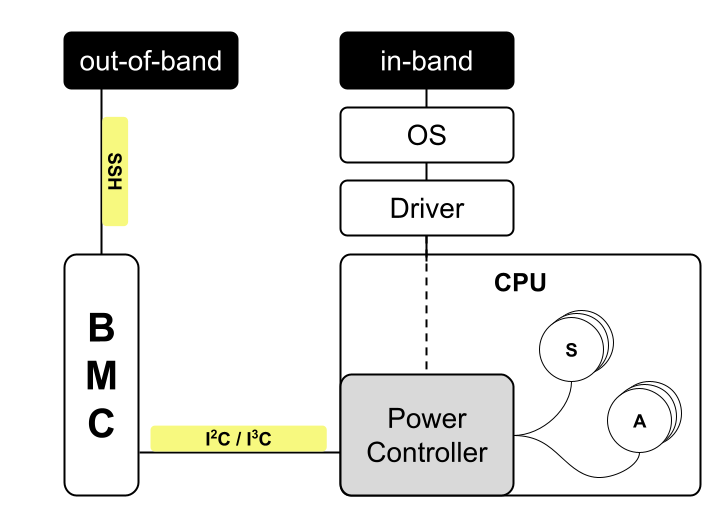
\includegraphics[width=0.5\textwidth]{img/SoA.png}
    \centering
    \caption{Differenza tra le interfacce in-band e out-of-band}\label{fig:SoAinoutband}
\end{wrapfigure}
accedere agli attuatori e sensori presenti nei core sia in modo diretto che da ''remoto''. Normalmente per farlo ci sono due vie disponibili basate su interfacce differenti:
\begin{itemize}
    \item in-band
    \item out-of-band
\end{itemize}
% Nella figura~\ref{fig:SoAinoutband} viene schematizzata la differenza tra le due interfacce disponibili. 
Nella figura~\ref{fig:SoAinoutband} viene schematizzato l'accesso ai dispositivi hardware che si occupano della gestione del power management su sistemi HPC. Sarebbe in realtà possibile accedere a questi componenti anche tramite altri meccanismi specifici, ad esempio la mappatura in memoria condivisa dei componenti hardware, tuttavia a causa della loro natura altamente specializzata, tali approcci non saranno considerati nell'ambito di questa tesi.

% I servizi in-band vengono forniti alle applicazioni e ai sistemi operativi in esecuzione negli elementi di elaborazione del chip e sono composti da: (i) governor dedicati alla potenza e telemetria correlata alla potenza a livello di sistema operativo; (ii) un'interfaccia dedicata per consentire alle applicazioni e ai tempi di esecuzione del modello di programmazione di specificare suggerimenti e prescrizioni per la gestione della potenza; (iii) un'interfaccia dedicata al Sistema e alla Gestione delle Risorse per supportare il capping della potenza a livello di CPU e nodo, nonché per gestire il compromesso tra Throughput ed Efficienza Energetica. I servizi out-of-band vengono forniti all'amministratore di sistema e agli strumenti di gestione del sistema tramite il Controller di Gestione della Scheda (BMC). Questi servizi consistono nella telemetria di potenza out-of-band, nel capping di potenza a livello di sistema e nella affidabilità e assistenza.

% (ii) off-chip ai Moduli Regolatori di Tensione (VRM) che alimentano il chip, gli altri componenti a bordo e il Controller di Gestione della Scheda (BMC).

\section{Servizi in-band}
I servizi in-band accedono alle risorse hardware tramite codice che esegue sul processore stesso. Questi sono resi possibili da infrastrutture come CPUfreq\cite{CPUfreq} o RAPL\cite{RAPL} (per architetture intel) che tramite dei driver, espongono a livello utente le manopole per gestire e monitorare frequenze e informazioni della cpu. Questo passaggio viene reso possibile da interfacce fornite dal sistema operativo. Queste ultime possono essere gestite in automatico in base al carico di sistema, in risposta ad eventi ACPI oppure in modo manuale. Una volta scelti i driver come \emph{ACPI CPUfreq driver} o \emph{Intel P-state} (in sistemi intel) è possibile scegliere tra diversi governors (o governatori) disponibili, che permettono di agire con delle policy differenti.
Per esempio \emph{CPUfreq} fornisce diversi governors per soddisfare diversi tipi di situazioni, come:
\begin{itemize}
    \item performance: forza la CPU ad eseguire alla frequenza massima disponibile;
    \item powersave: forza quella minima;
    \item ondemand: comportamento dinamico in base all'utilizzo di sistema;
    \item userspace: permette ai selezionati user-space di impostare la frequenza; 
    \item conservative: come ondemand ma con più inerzia al cambiamento;
\end{itemize}

\begin{figure}[H]
    \centering
    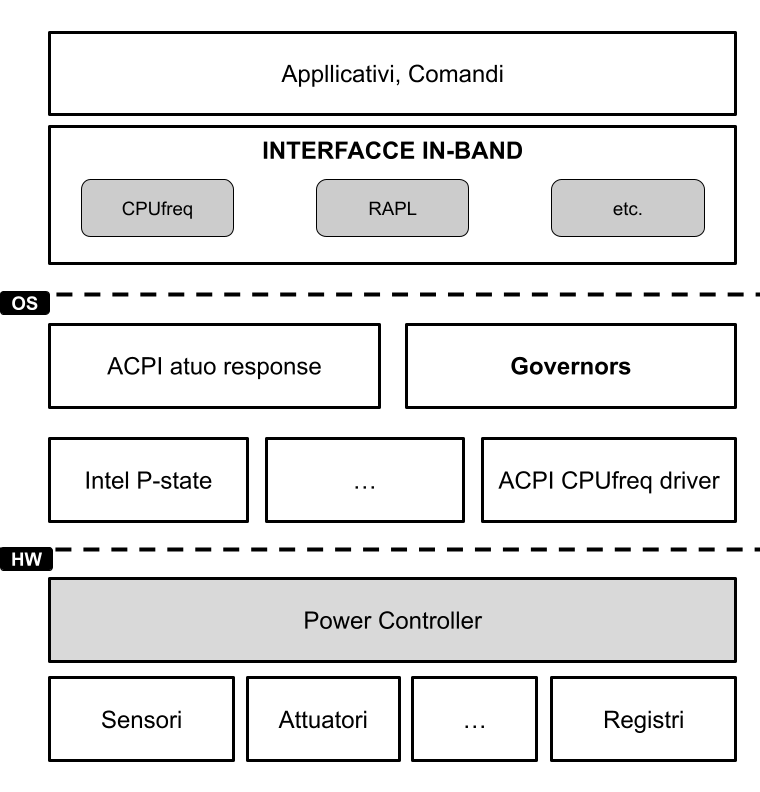
\includegraphics[width=0.65\textwidth]{img/in-band.png}
    \caption{Struttura interfacce in-band: divise su più livelli tra cui Sistema Operativo (SO) e Hardware (HW)}\label{fig:inband}
\end{figure}

Il vantaggio di usare queste interfacce è che permettono di operare in real-time ed in modo dinamico. I lati negativi invece risiedono nelle stesse peculiarità di questi strumenti, ovvero che possono ottenere le informazioni solamente nei core sui quali i processi vengono eseguiti. 

% E' reso possibili tramite degli specifici driver (intel\_pstate) che comunicano con i componenti hardware sul chip. Diversamente \textbf{Intel Power Governors} utilizza le interfacce proprietarie (RAPL) con cui monitora potenza ed energia a livello di sistema.
% Entrambi questi strumenti hanno necessità di componenti Hardware dedicati come i power knob (manopole per la gestione della potenza) e sensori che permettono di monitorare temperature e tensioni.
% I servizi in-band sono molto flessibili e permetto di operare in real-time ed in modo dinamico. Infatti interagendo con l' Hardware e passando tramite il sistema operativo, sono necessari semplici chiamate e comandi per controllare questi strumenti.

\section{Servizi out-of-band}
Contrariamente alle interfacce in-band, i servizi out-of-band fanno utilizzo di \emph{sidechannels} ovvero canali di accesso alternativi per ottenere i dati richiesti. Questo meccanismo permette a processi esterni\footnote{In esecuzione su processori diversi dai quali si vuol reperire dati} di accedere alle informazioni contenute nel processore che si vuole analizzare. Per di più questo permette di monitorare i componenti anche quando ci sono errori ed eccezioni che normalmente bloccherebbe il servizio. Un componente tra i più importanti che svolge questa funzione è il Baseboard Management Controller (BMC), solitamente un micro-controllore animato da sistemi embedded linux, e accessibile tramite un canale separato (solitamente provvisto di una propria interfaccia di rete e/o bus specifici). Il suo principale scopo è quello di monitorare in modo dettagliato lo stato di tensioni, temperature, ventole e prestazioni dei processori e fornire contemporaneamente servizi di power capping sia a livello di sistema (non possibile tramite le interfacce in-band) che di singoli processori.
Recentemente alcuni produttori di BMC introducono anche dispositivi FPGA da affiancare al BMC per aumentarne le capacità.
% \vfil
\begin{figure}[H]
    \centering
    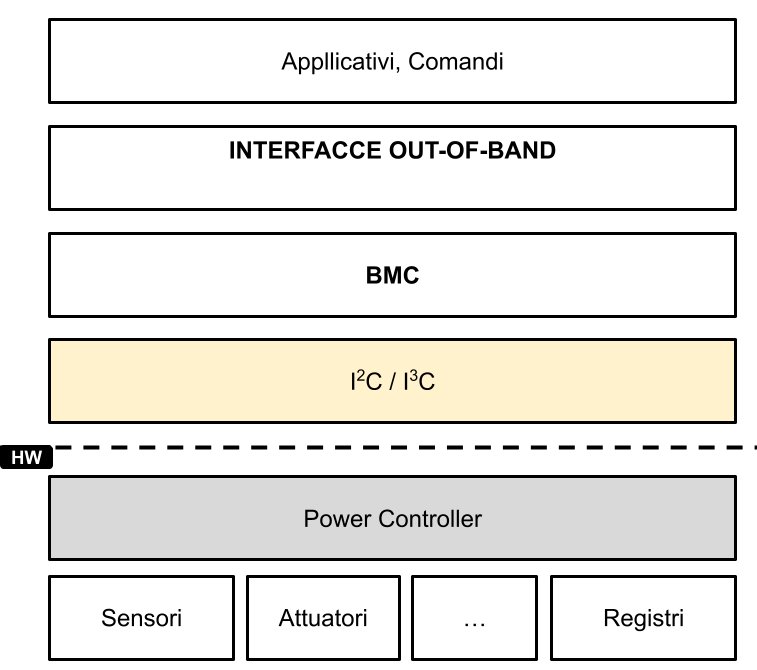
\includegraphics[width=0.75\textwidth]{img/out-of-band.png}
    \caption{Struttura interfacce out-of-band} 
    \label{fig:out-of-band}
\end{figure}


\section{Interfacce di alto livello}
Nel corso degli anni con l'obbiettivo di ottimizzare e automatizzare l'interazione con questi meccanismi hardware sono stati sviluppati diversi software di più alto livello che utilizzano sia interfacce in band che interfacce out of band. Si possono ricordare i più famosi: \emph{Variorum} (LLNL), \emph{GEOPM} (Intel)\cite{GEOPM}, e \emph{HDEEM} (Atos)\cite{HDEEM}. Tutti questi rappresentano però un tentativo di fornire una soluzione ad un sottoinsieme di problemi per la gestione dell'energia o potenza, piuttosto che ad un software con visione globale di Power Management per sistemi di calcolo ad alte prestazioni. %MANCANZA DI VISIONE GLOBALE!!!


\section{Modello di power stack} %Componenti power stack
Con Power Stack si intende un insieme di software che cooperando riescono a fornire ad applicazioni, utenti e amministratori la gestione completa del Power Management. Una volta definito il problema, ed i componenti che possono essere utilizzati, è possibile definire un modello di interazione e responsabilità dei vari attori. Di seguito vengono riportati quelli che sono i ruoli necessari al fine di coordinare un sistema HPC dall'allocazione di un applicativo, fino alla gestione delle tensioni. 
\begin{itemize}
    \item Workflow engine (WE)
    \item System Power Manager (SPM)
    \item Job Manager (JM)
    \item Job Scheduler (JS)
    \item Resource Manager (RM)
    \item Node Manager (NM)
    \item Monitor (M)
\end{itemize}
%TODOV aggiungi i tipi di informazioni che si scambiano, per facilitare nel modello la realizzazione

\subsection{Workflow engine}
Il workflow o \emph{flusso di lavoro} è un insieme task che devono essere svolti per risolvere un determinato problema. Il workflow engine si occupa di analizzare le dipendenze e le richieste di risorse di ogni workflow e decide dinamicamente come dividerlo nei jobs che verranno successivamente assegnati al Job Scheduler. %Si occupa quindi di analizzare ed assegnare i diversi task a chi poi va ad eseguirli.

\subsection{System Power Manager}
Il System Power Manager si occupa di comunicare con tutti i Node Manager all'interno del sistema, per impostare eventuali limiti di potenza. Questi ultimi vengono solitamente impostati manualmente dagli amministratori di sistema, oppure in modo automatico comunicando con altri attori, come monitor e Node Manager. Una volta fissati i limiti, vengono monitorati i dati relativi a potenza ed energia, e controlla di conseguenza i budget, e la \emph{user-fairness}.
\subsection{Job scheduler}
%Il System Manager
Il job scheduler dopo aver ricevuto come input un insieme di jobs li schedula all'interno del sistema, e in modo indicativo decide quando schedulare ogni job, su quale nodo, e con quale power budget. In particolare la serie di compiti che si trova a svolgere è il seguente:
\begin{enumerate}
    \item L'utente schedula i jobs da svolgere in una o più code, definite dal Workflow Engine.
    \item Il Job scheduler esamina tutte le code e i job in esse contenute, e decide dinamicamente, quale sarà l'ordine di esecuzione, e il tempo massimo in cui viene assegnata una risorsa.
\end{enumerate}
Generalmente si cerca di ottimizzare alcune caratteristiche come il tempo di utilizzo del sistema oppure l'accesso veloce alle risorse per alcuni sottoinsiemi di jobs. Inoltre le code definite, possono avere diverse priorità o può essere ristretto l'accesso a soli alcuni utenti.% I job scheduler possono condividere un nodo anche con più utenti contemporaneamente, in base all'utilizzo che devono farne. Per farlo il nodo viene allocato e diviso in partizioni virtuali, che vengo ''sciolte'' una volta finiti i job in esecuzione. Questo permette di utilizzare al massimo i componenti messi a disposizione dal sistema HPC.

\subsection{Resource Manager}
Per riuscire a svolgere questo lavoro il Job Scheduler interagisce con uno o più Resource Manager\footnote{A volte per questo il Job Manager ed il Resource Manager vengono collassati in un unico componente}. Questi sono software che hanno il compito di dividere (o condividere) e orchestrare le risorse computazionali e fisiche del sistema HPC. Queste risorse includono diversi componenti:
\begin{itemize}
    \item Nodi
    \item Processori
    \item Memorie
    \item Dischi
    \item Canali di comunicazione (compresi quelli di I/O)
    \item Interfacce di rete 
\end{itemize}
Per esempio quando un Job Scheduler deve eseguire un job, richiede al RM di allocare core, memorie, dischi e risorse di rete in base alle specifiche di esecuzione del job.
Infine in alcuni casi il RM è anche responsabile di gestire la distribuzione elettrica e raffreddamento di alcune parti dei centri di calcolo\cite{ResourceManager}.

\subsection{Job Manager}
Lo scopo del job manager è quello di effettuare ottimizzazioni job-centriche considerando le prestazioni di ogni applicazioni, il suo utilizzo di risorse, la sua fase e qualsiasi interazione dettata da ogni workflow in cui è presente. In breve il job manager decide i target delle manopole del Power Management, come (i) CPU power cap, (ii) CPU clock frequency oltre ad eseguire ottimizzazione del codice.

\subsection{Node Manager}
Il node manager fornisce accesso ai controlli e monitoraggio hardware a livello del nodo. Volendo permette anche di definire delle policy di power management. Ha infine lo scopo di preservare integrità, sicurezza del nodo sia in termini informatici che fisici.

\subsection{Monitor}

Il monitor è responsabile di collezionare tutte le metriche in-band e out-of-band che riguardando prestazioni, utilizzo e stato delle risorse, potenza ed energia.
Tutto questo deve essere fatto con il minor impatto possibile sul sistema dove sta agendo, collezionando, aggregando e analizzando le metriche e dove necessario, scambiandole ad altri attori. A sua volta il \emph{Monitor} è scomponibile in tre sotto-moduli:
\begin{itemize}
    \item Gestione Firma che genera una firma che identifica univocamente il job; 
    \item Estimatore che valuta le proprietà dei job o dello stato del sistema usando la firma generata precedentemente;
    \item Dashboard che fornisce le funzionalità da mostrare agli sviluppatori.
\end{itemize}


Per concludere viene mostrato uno schema in figura~\ref{fig:powerstackscheme} che mostra gli attori e le possibili interazioni che possono avere.
\begin{figure}[H]
    \centering
    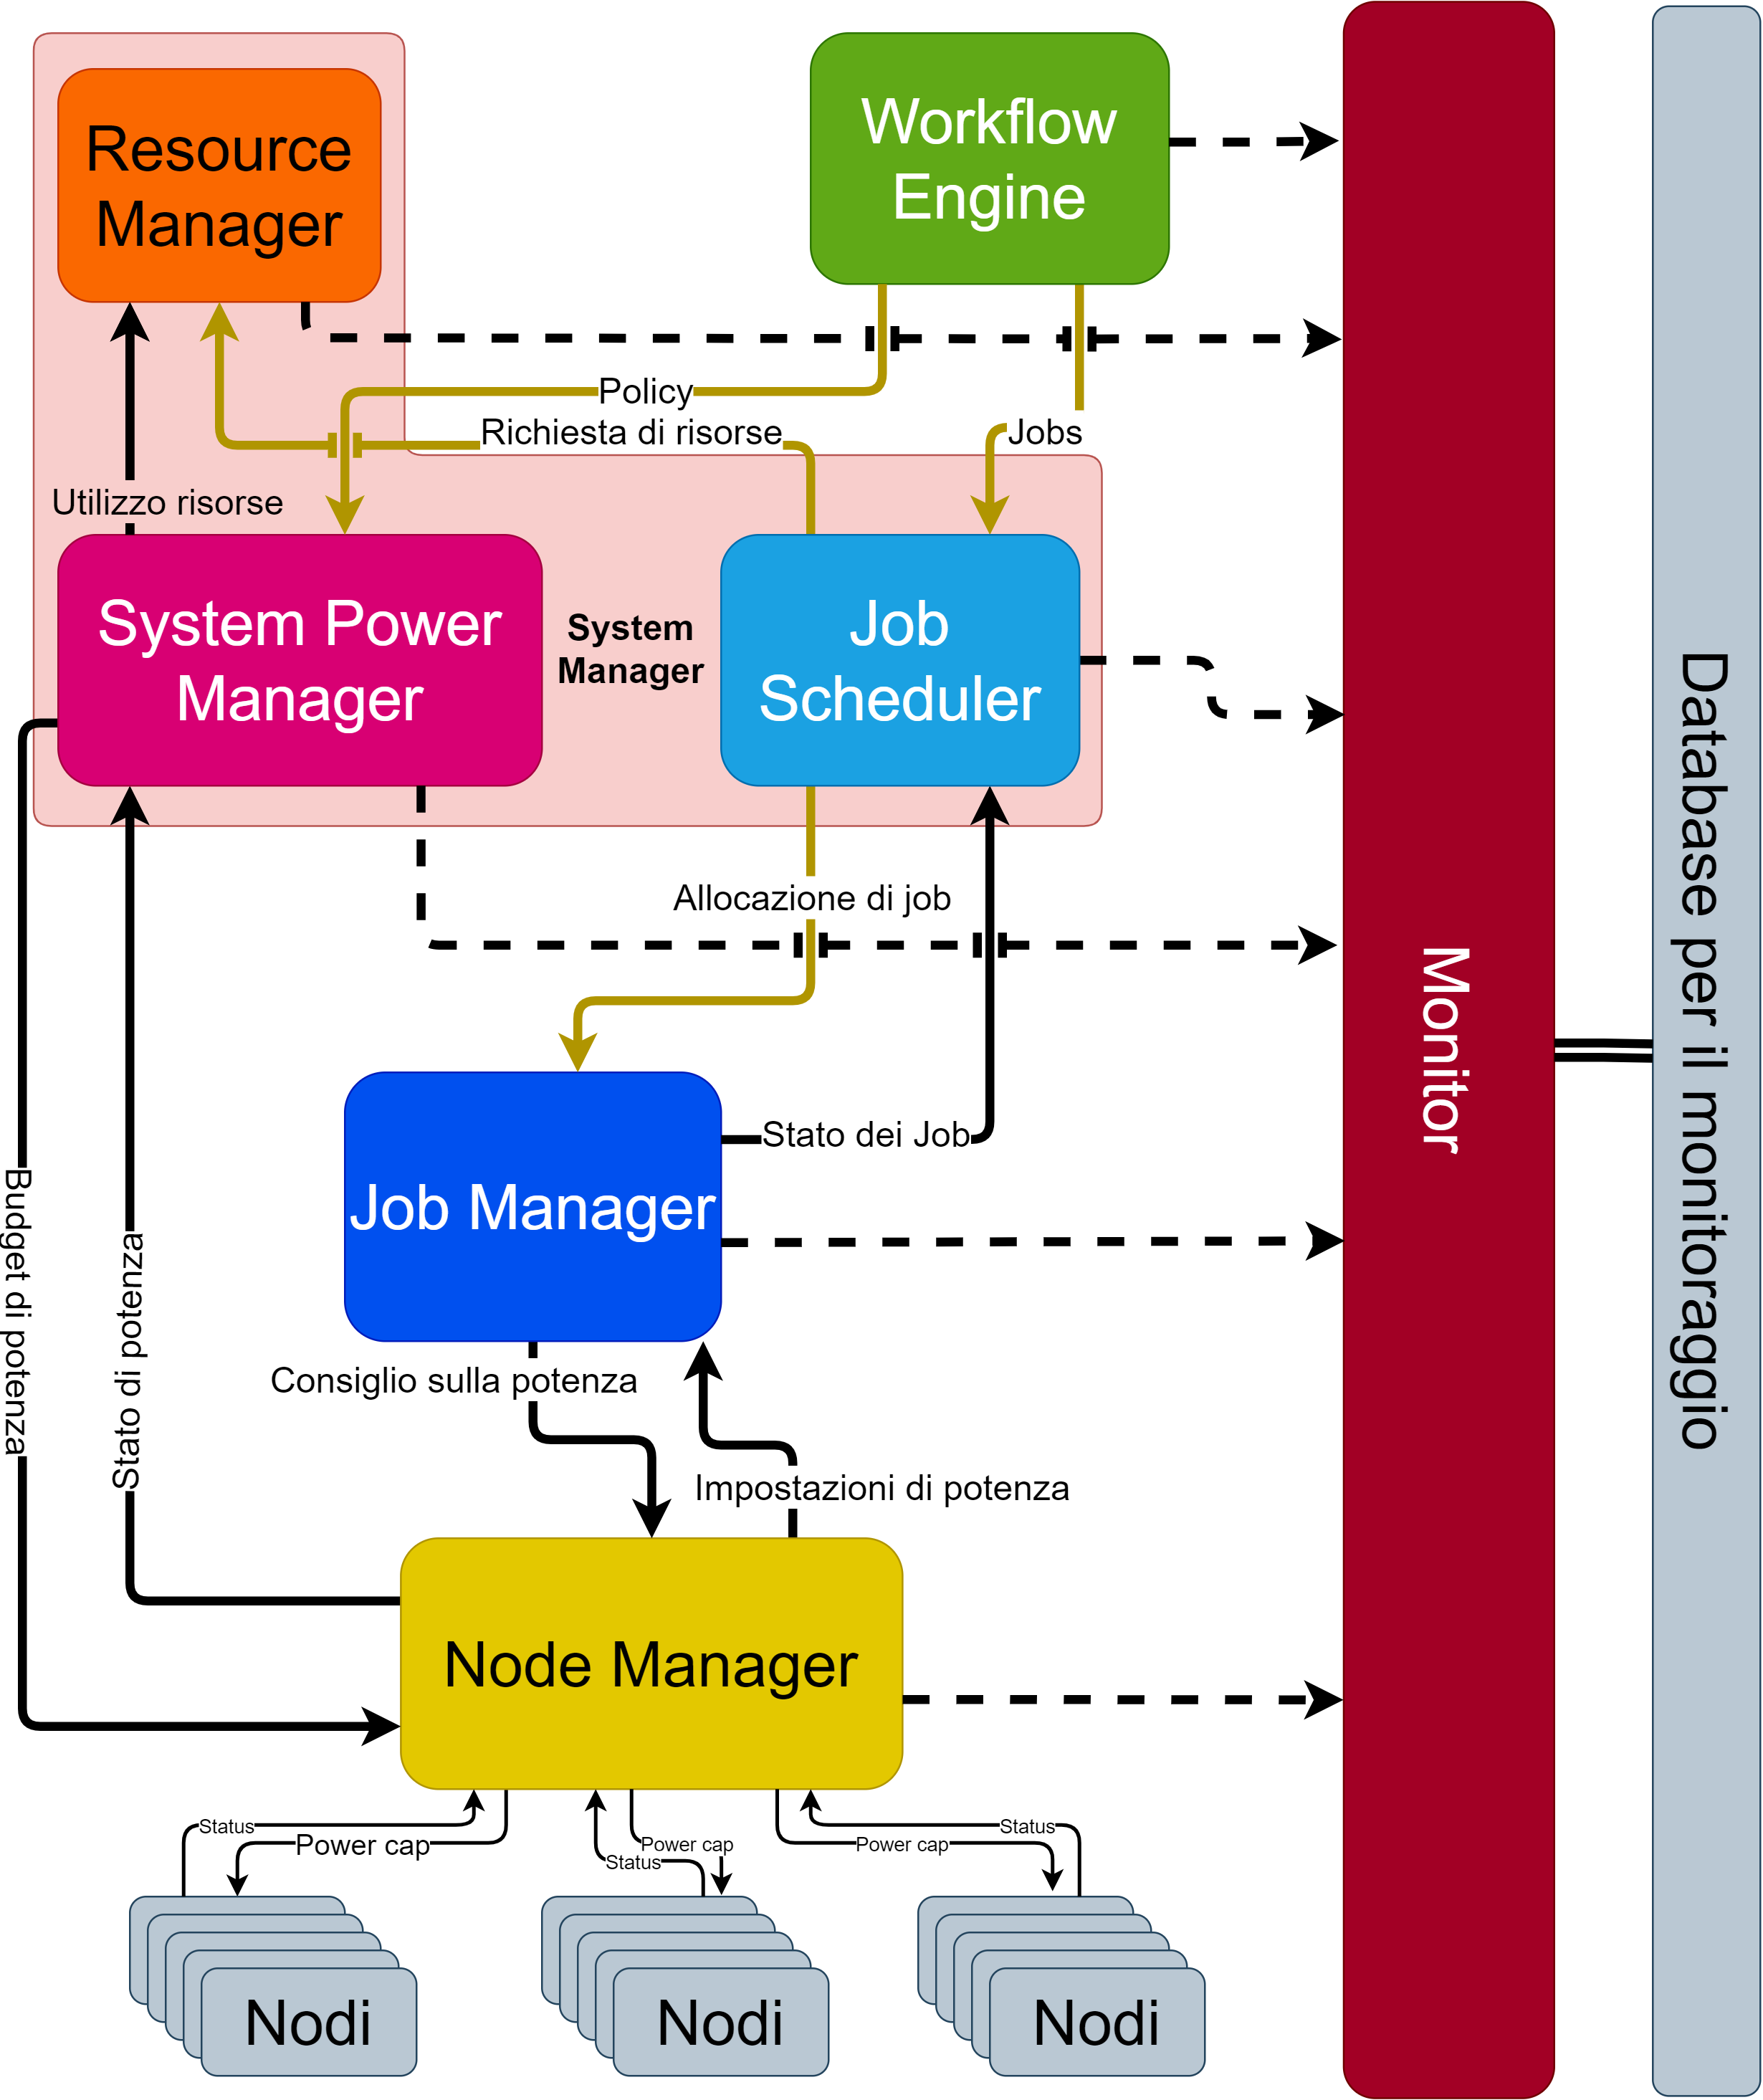
\includegraphics[width=\textwidth]{img/SchemaPowerStack.drawio.png}
    \caption{Modello di power stack}\label{fig:minpowerstackscheme}
\end{figure}



\chapter{DDS \& RTPS}\label{Chapter:dds}
DDS (Data Distribution Service)\cite{DDS} e RTPS (Real-Time Publish-Subscribe)\cite{RTPS} costituiscono due soluzioni fondamentali nel campo delle comunicazioni distribuite e real-time. Queste tecnologie svolgono un ruolo importante nella la trasmissione di dati tra dispositivi e applicazioni interconnesse, rivestendo particolare importanza in scenari complessi come i sistemi embedded, e ad alte prestazioni come HPC. 


\section{Implementazione usasta}
DDS e RTPS sono dei protocolli di comunicazione per specifici casi di utilizzo. Ci sono state diverse implementazioni di questi protocolli da diversi società e organizzazioni, come:
\begin{itemize}
  \item FastDDS (eprosima)
  \item CycloneDDS (Oracle)
  \item ConnextDDS
  \item GurumDDS
\end{itemize}

e tante altre. In tutti i successivi capitoli verrà preso come riferimento FastDDS ed in particolare la sua versione 2.11.2 \cite{FastDDS}. E' stato scelto di utilizzare questa implementazione  dato il supporto per le comunicazione Real-Time, e le impostazioni delle Qualità del servizio(QoS) che la rendevano adeguatamente configurabile per un utilizzo su sistemi di HPC. %TODO: Da migliorare

\section{DDS}
Data Distribution Service è un protocollo di comunicazione incentrato sullo scambio di dati per sistemi distribuiti. Questo si basa su modello chiamato Data-Centric Publish Subscribe (DCPS). I principali attori che vengono coinvolti sono:
\begin{itemize}
    \item Publisher: responsabile della creazione e configurazione dei DataWriter. Il DataWriter è l'entità responsabile della pubblicazione effettiva dei messaggi. Ciascuno avrà un Topic assegnato sotto il quale vengono pubblicati i messaggi;\label{actor:publisher}

    \item Subscriber: responsabile di ricevere i dati pubblicati sotto i topic ai quali si iscrive. Serve uno o più oggetti DataReader, che sono responsabili di comunicare la disponibilità di nuovi dati all'applicazione;\label{actor:subscriber}

    \item Topic: collega i DataWriter con i DataReader. È univoco all'interno di un dominio DDS;\@
    
    \item Dominio: utilizzato per collegare tutti i publisher e subscriber appartenenti a una o più domini di appartenenza, che scambiano dati sotto diversi topic. Il DomainParticipant funge da contenitore per altre entità DCPS, e svolge anche la funzione di costruttore di entità Publisher, Subscriber e Topic fornendo anche servizi di QoS;\@

    \item Partizione: costituisce un isolamento logico di entità all'interno dell'isolamento fisico offerto dal dominio;

\end{itemize}
Inoltre DDS definisce le cosidette Qualità di Servizio (QoS policy) che servono configurare il comportamento di ognuno di questi attori.


\section{RTPS}
Real-Time Publisher Subscribe è un middleware\footnote{Formalmente è un protocollo a se stante, utilizzato da DDS come middlware} utilizzato da DDS per gestire la comunicazione su diversi protocolli di rete come UDP/TCP e Shared Memory. Il suo principale scopo è quello di inviare messaggi real-time, con un approccio best-effort e cercando di massimizzare l'efficienza. E' inoltre progettato per fornire strumenti per la comunicazione unicast e multicast. Le principali entità descritte da RTPS sono:
\begin{itemize}
    \item RTPSWriter: endpoint capace di inviare dati;
    \item RTPSReader: endpoint abilitato alla ricezione dei dati;
\end{itemize}
Ereditato da DDS anche RTPS ha la concezione di Dominio di comunicazione e come questo, le communcazioni a livello di RTPS girano attorno al concetto di Topic prima definito. L'unità di comunicazione è chiamata \textbf{Change} che rappresenta appunto un cambiamento sui dati scritti sotto un certo topic. Ognuno degli attori registra questi \emph{Change} in una struttura dati che funge da cache.
In particolare la sequenza di scambio è:
\begin{enumerate}
    \item il \emph{change} viene aggiunto nella cache del RTPSWriter;
    \item RTPSWriter manda questa \emph{change} a tutti gli RTPSReader che conosce;
    \item quando RTPSReader riceve il messaggio, aggiorna la sua cache con il nuovo \emph{change}.
\end{enumerate}

\begin{figure}[H]
    \centering
    \begin{subfigure}{0.45\linewidth}
      \centering
      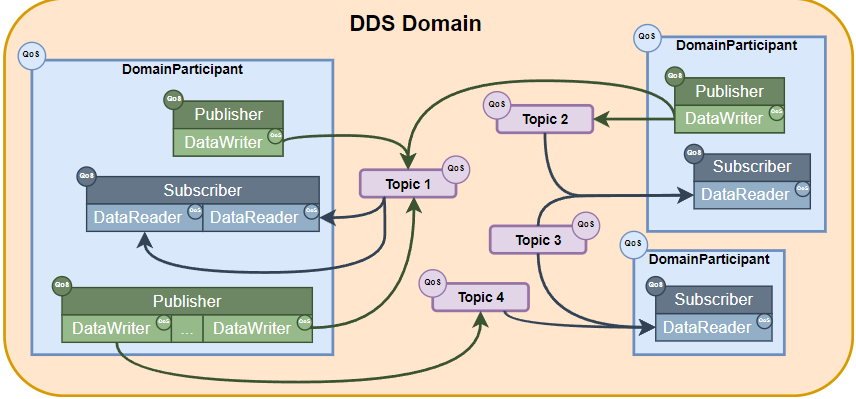
\includegraphics[width=\linewidth]{./img/dds_architecture.png}
      \caption{Schema DDS}\label{fig:dds}
    \end{subfigure}
    \begin{subfigure}{0.45\linewidth}
      \centering
      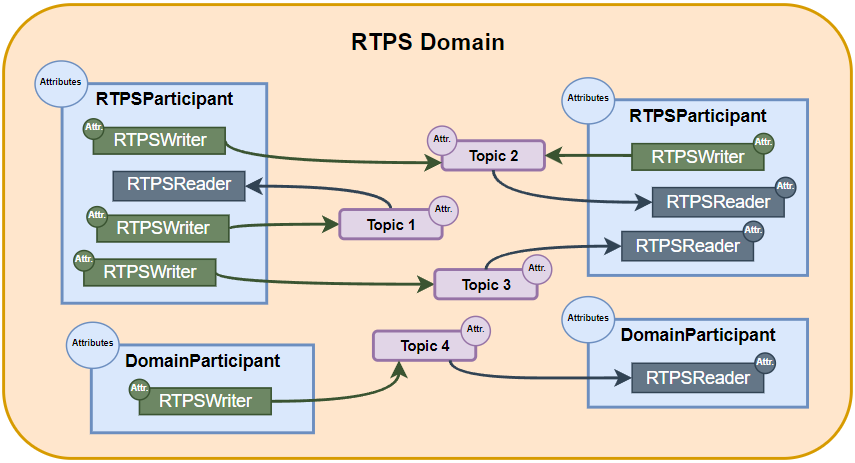
\includegraphics[width=\linewidth]{./img/rtps_architecture.png}
      \caption{Schema RTPS}\label{fig:rtps}
    \end{subfigure}
    \caption{Confronto tra architettura DDS e RTPS}\label{fig:confrontodds_rtps}
  \end{figure}

%TODO: ROS

\section{ROS}\label{SSEC:rosiface}


Questo approccio distribuito per la distribuzione dei dati tra vari attori utilizzando un middlware basato su DDS non è idea inedita. Infatti dalla sua seconda versione il software open-source \textbf{Robot Operating System} meglio conosciuto come ROS
\begin{wrapfigure}{r}{0.5\textwidth}
  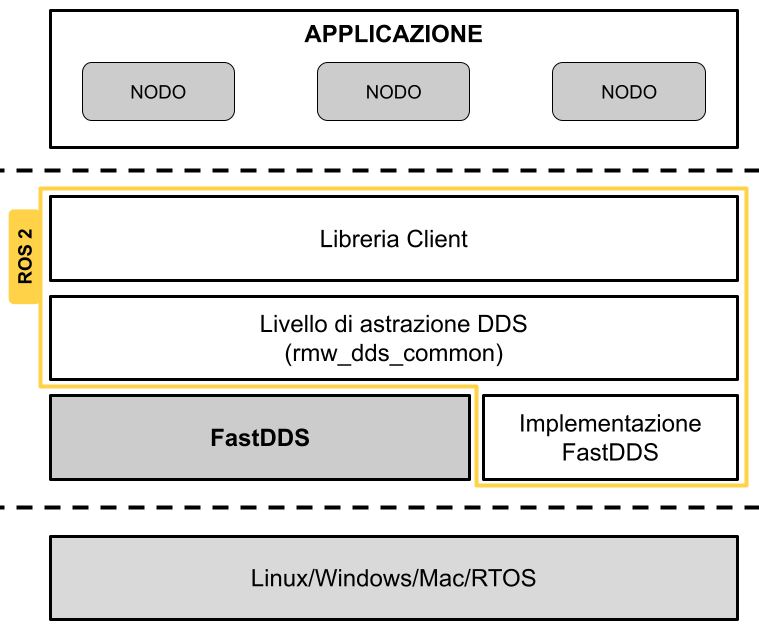
\includegraphics[width=0.5\textwidth]{img/ROS_MW.png}
  \caption{Ros Middleware per DDS} 
  \label{fig:rmw_dds_common}
\end{wrapfigure}
ha deciso di usare questi strumenti introducendo un ulteriore livello che permette di usare diverse implementazioni di DDS. Questa idea è stata e sarà di grande ispirazione per il completamento di questo progetto.
Nello specifico, è stata creata una libreria chiama rmw\_dds\_common(ros middleware) come mostrato nella \ref{fig:rmw_dds_common}\footnote{L'implementazione di FastDDS vuole essere un esempio tra le diverse soluzioni disponibili per ROS2} sopra il quale la community ha creato le implementazioni di DDS desiderate, andando a creare così diverse possibilità di configurazione dello stesso servizio di distribuzione dati.
Inoltre per cambiare tra le diverse versioni di DDS si deve semplicemente impostare una variabile di ambiente, rendendo il procedimento facile per tutti i possibili fruitori di ROS2. 

Tuttavia è stato scelto di utilizzare direttamente l'implementazione DDS invece che \emph{Ros middlware} per i seguenti motivi:
\begin{itemize}
    \item Potenzialità: ROS mette a disposizione solo alcuni degli strumenti resi disponibili dallo strato DDS, andando a limitare la possibilità di sfruttamento di tutte le impostazioni e QoS di FastDDS;
    \item Granularità: oltre alla mancanza di alcune funzionalità, in ros sono predisposti dei pacchetti preconfigurati di entità. Per andare a studiare più approfonditamente gli strumenti su architetture diverse, è più pratico avere la possibilità di cambiare ogni piccola configurazione.
    \item Flessibilità: Per andare a definire delle strutture dati di ROS, al fine di scambiare messaggi DDS usando il middleware offerto, era necessario creare diverse strutture dati che combaciassero con le interfacce ROS;
    \item Diversa natura: In ROS, la maggior parte delle comunicazioni fatte sono intra-processo e raramente viene utilizzata una infrastruttura di rete, per andare a collegare tutti i nodi. Per questo sono maggiormente ottimizzate quel tipo di comunicazioni, piuttosto che quelle su rete, come in questo caso.
    \item Facilità di implementazione: Implementare completamente \emph{rmw\_dds\_common} richiedeva un impegno e uno studio non indifferente della architettura sottostante a ROS, che seppur ben documentata, sarebbe costata diverso tempo. 
\end{itemize}


% in ROS, la maggior parte delle comunicazioni fatte sono intra-processo e raramente viene utilizzata una infrastruttura di rete, per andare a scambiare dei messaggi. Per questo sono maggiormente ottimizzate quel tipo di comunicazioni, piuttosto che quelle su rete, come nel caso di HPC


% Ros Middleware interface\cite{ros2iface}, developed within the context of the Robot Operating System (ROS), stands as a pinnacle of innovation in the realm of creating middleware for Distributed Data Systems. The middleware leverages advanced data serialization techniques, optimized for real-time performance and efficient data exchange. Its incorporation of Quality of Service parameters and support for both publish-subscribe and request-response communication patterns underscores its sophistication, making it a state-of-the-art choice for building DDS middleware in distributed environments.

% In fact ROS capitalizes on the Data Distribution Service as a foundational communication middleware protocol\cite{ros2iron}, which plays a pivotal role in enabling seamless and efficient data exchange and interaction between the myriad components that constitute a robotic ecosystem.

% The structure of the middleware-ROS, exemplified by \emph{rmw\_dds\_common}\cite{ros2iron}, combined with various middleware specific to each DDS service provider, also allows for easy switching of the DDS implementation using a simple variable change, invoked before launching the ROS-node, among the many available options (FastDDS, CycloneDDS, ConnextDDS, etc.). 
% This approach permits choosing the most suitable DDS implementation for specific use case. For instance, if we intend to use FastDDS (most suitable one for real-time communications) as the primary DDS service, we can set \emph{rmw\_implementation=fastdds}, and ROS will be able to abstract all of its functions.
\chapter{REGALE}\label{chap:4_REGALE}
%COSA
REGALE\cite{REGALE} è un progetto finanziato dall'UE\cite{ue_REGALE} nato ad Aprile 2021 che opera nell'ambito del Power Management in sistemi ad High-Performance Computing ed in particolare si è focalizzato su sistemi Exascale\footnote{Exascale: capace di eseguire operazioni nell'ordine di ExaFlops ($10^{18}$)}.

\section{Obbiettivi}
Il loro principale obbiettivo è aprire la strada alla prossima generazione di applicazioni per HPC, riunendo importanti parti interessate, accademici e centri europei di supercalcolo. Il progetto si pone di definire un'architettura open-source con l'intenzione di costruire un prototipo in grado di dotare i sistemi di HPC dei meccanismi e delle politiche necessari per garantire un utilizzo delle risorse efficace\cite{ue_REGALE}. Per farlo sono inoltre state definite delle politiche da rispettare durante lo sviluppo di tutto il progetto:
\begin{itemize}
    \item Effettivo utilizzo delle risorse disponibili, tramite aumento del throughput del sistema e la minimizzazione della \emph{Performance Degradation} sotto vincoli di potenza;
    \item Ampia applicabilità attraverso l'inseguimento di concetti come scalabilità, indipendenza dalle piattaforme ed estensibilità;
    \item Facilità di implementazione tramite la creazione di una infrastruttura flessibile, e che gestisca in automatico le risorse.
\end{itemize}


\section{Power Stack}
L'intero progetto, durante il suo sviluppo si è basato su strumenti come MPI library\cite{mpi}, SLURM\cite{slurm}, o DCDB\cite{dcdb}. Inoltre, è stato deciso di introdurre software open-source che potessero soddisfare le esigenze del modello di Power Stack~\ref{fig:powerstackscheme}. Infatti sono stati valutati e selezionati diversi applicativi (molti dei quali prodotti dai partner, come mostrati in tabella~\ref{table:REGALE}) anche con ruoli analoghi, per soddisfare diverse esigenze.
\begin{table}[ht]
    \centering
    \begin{tabular}{l|l|l}
    \hline
    \textbf{Tool} & \textbf{Partner} & \textbf{Ruolo all'interno di REGALE} \\
    \hline
    SLURM & TUM & System Manager \\
    \hline
    OAR & UGA & System Manager \\
    \hline
    DCDB & LRZ & Monitor, Monitoring Data \\
    \hline
    BEO & ATOS & Monitor, Node Manager, Monitoring Data \\
    \hline
    BDBO & ATOS & Monitor, Job Manager \\
    \hline
    EAR & BSC & Monitor, Node Manager, Job Manager, Monitoring Data \\
    \hline
    Melissa & UGA & Workflow Engine \\
    \hline
    RYAX & RYAX & Workflow Engine \\
    \hline
    Examon & E4/UNIBO & Monitor, Monitoring Data \\
    \hline
    COUNTDOWN & CINECA/UNIBO & Job Manager \\
    \hline
    PULPcontroller & UNIBO & Node Manager \\
    \hline
    BeBiDa & RYAX & System Manager \\
    \hline
\end{tabular}
\caption{Software introdotti all'interno di REGALE con il partner che li ha prodotti e il loro ruolo}\label{table:REGALE}
\end{table}

\begin{figure}[htbp][H]
    \centering
    \begin{subfigure}[b]{0.45\textwidth}
    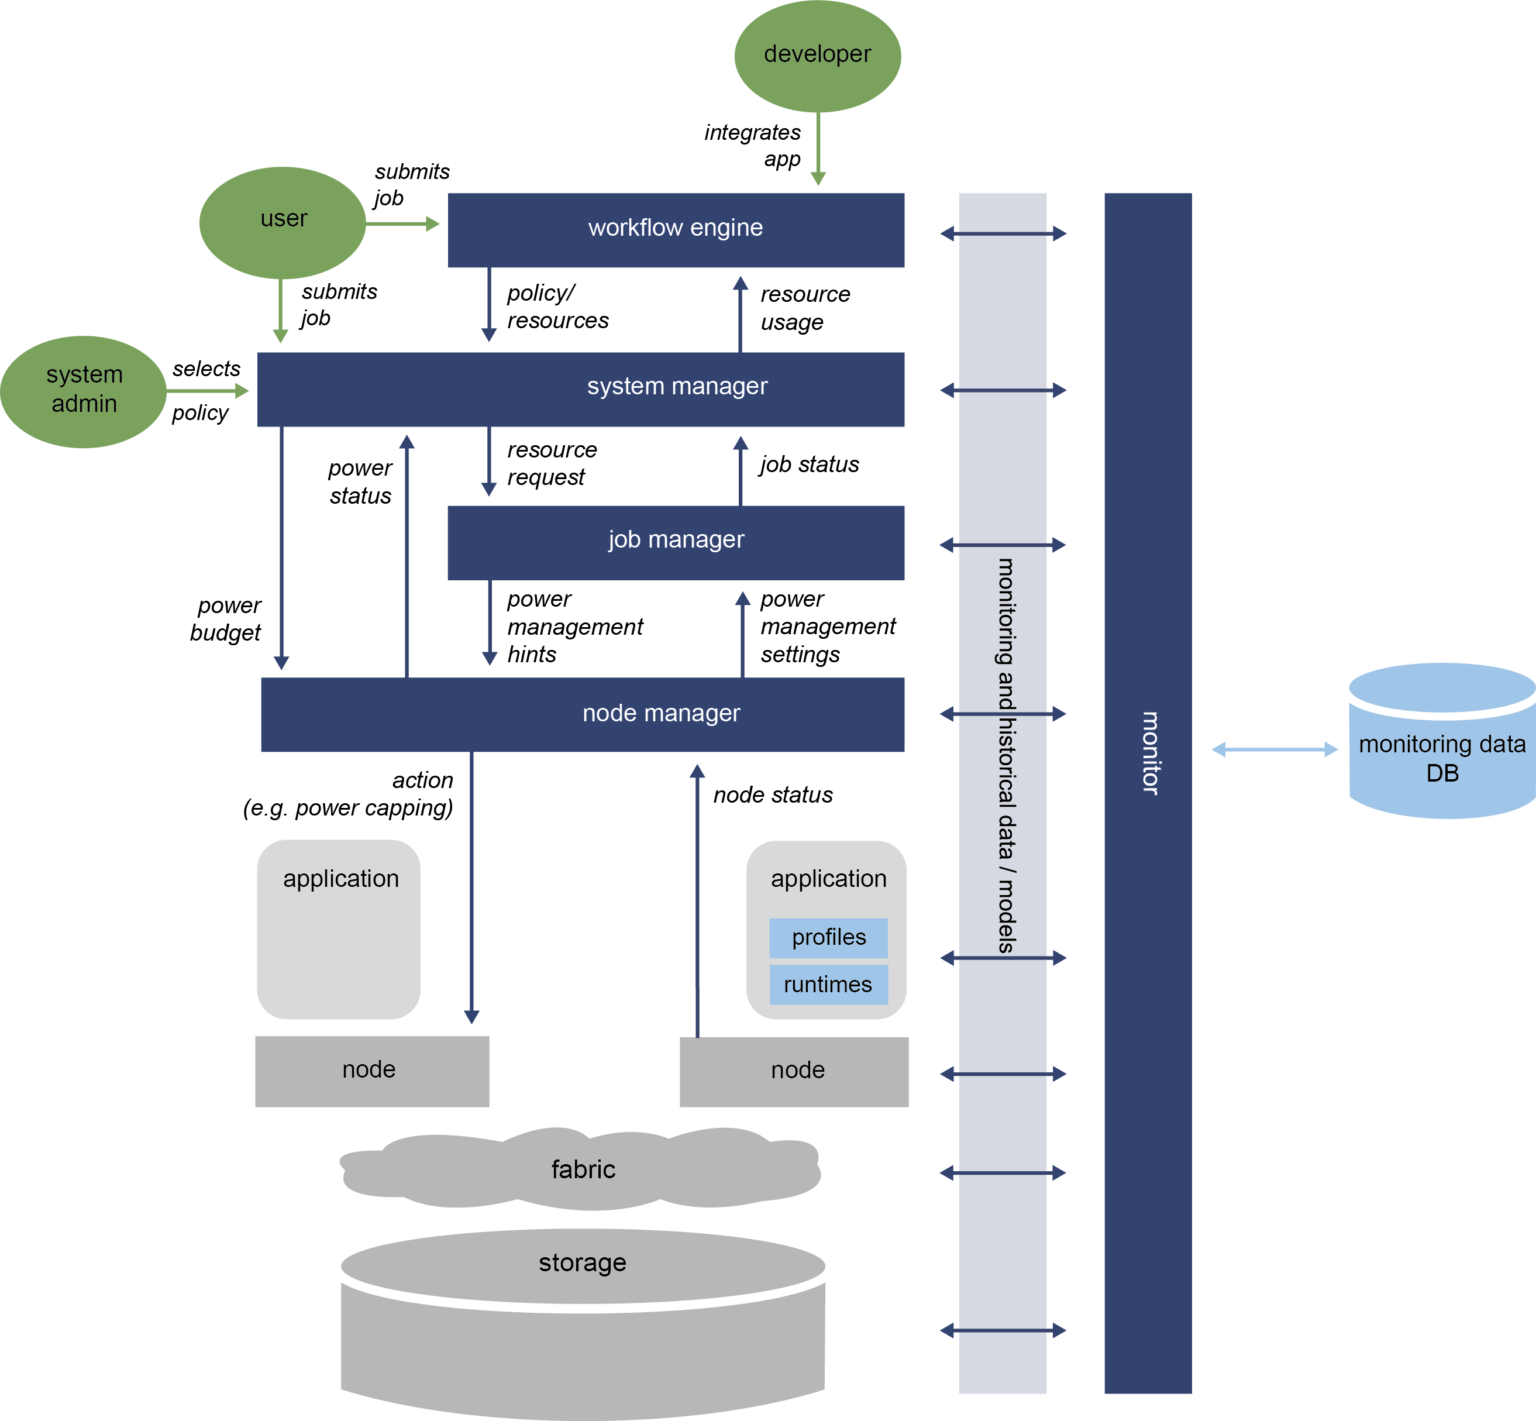
\includegraphics[width=\textwidth]{img/REGALE-Architecture-1536x1421.png}
    \caption{Modello di Power Stack Regale}\label{fig:powerstackscheme}
    \end{subfigure}
    \hfill
    \begin{subfigure}[b]{0.45\textwidth}
    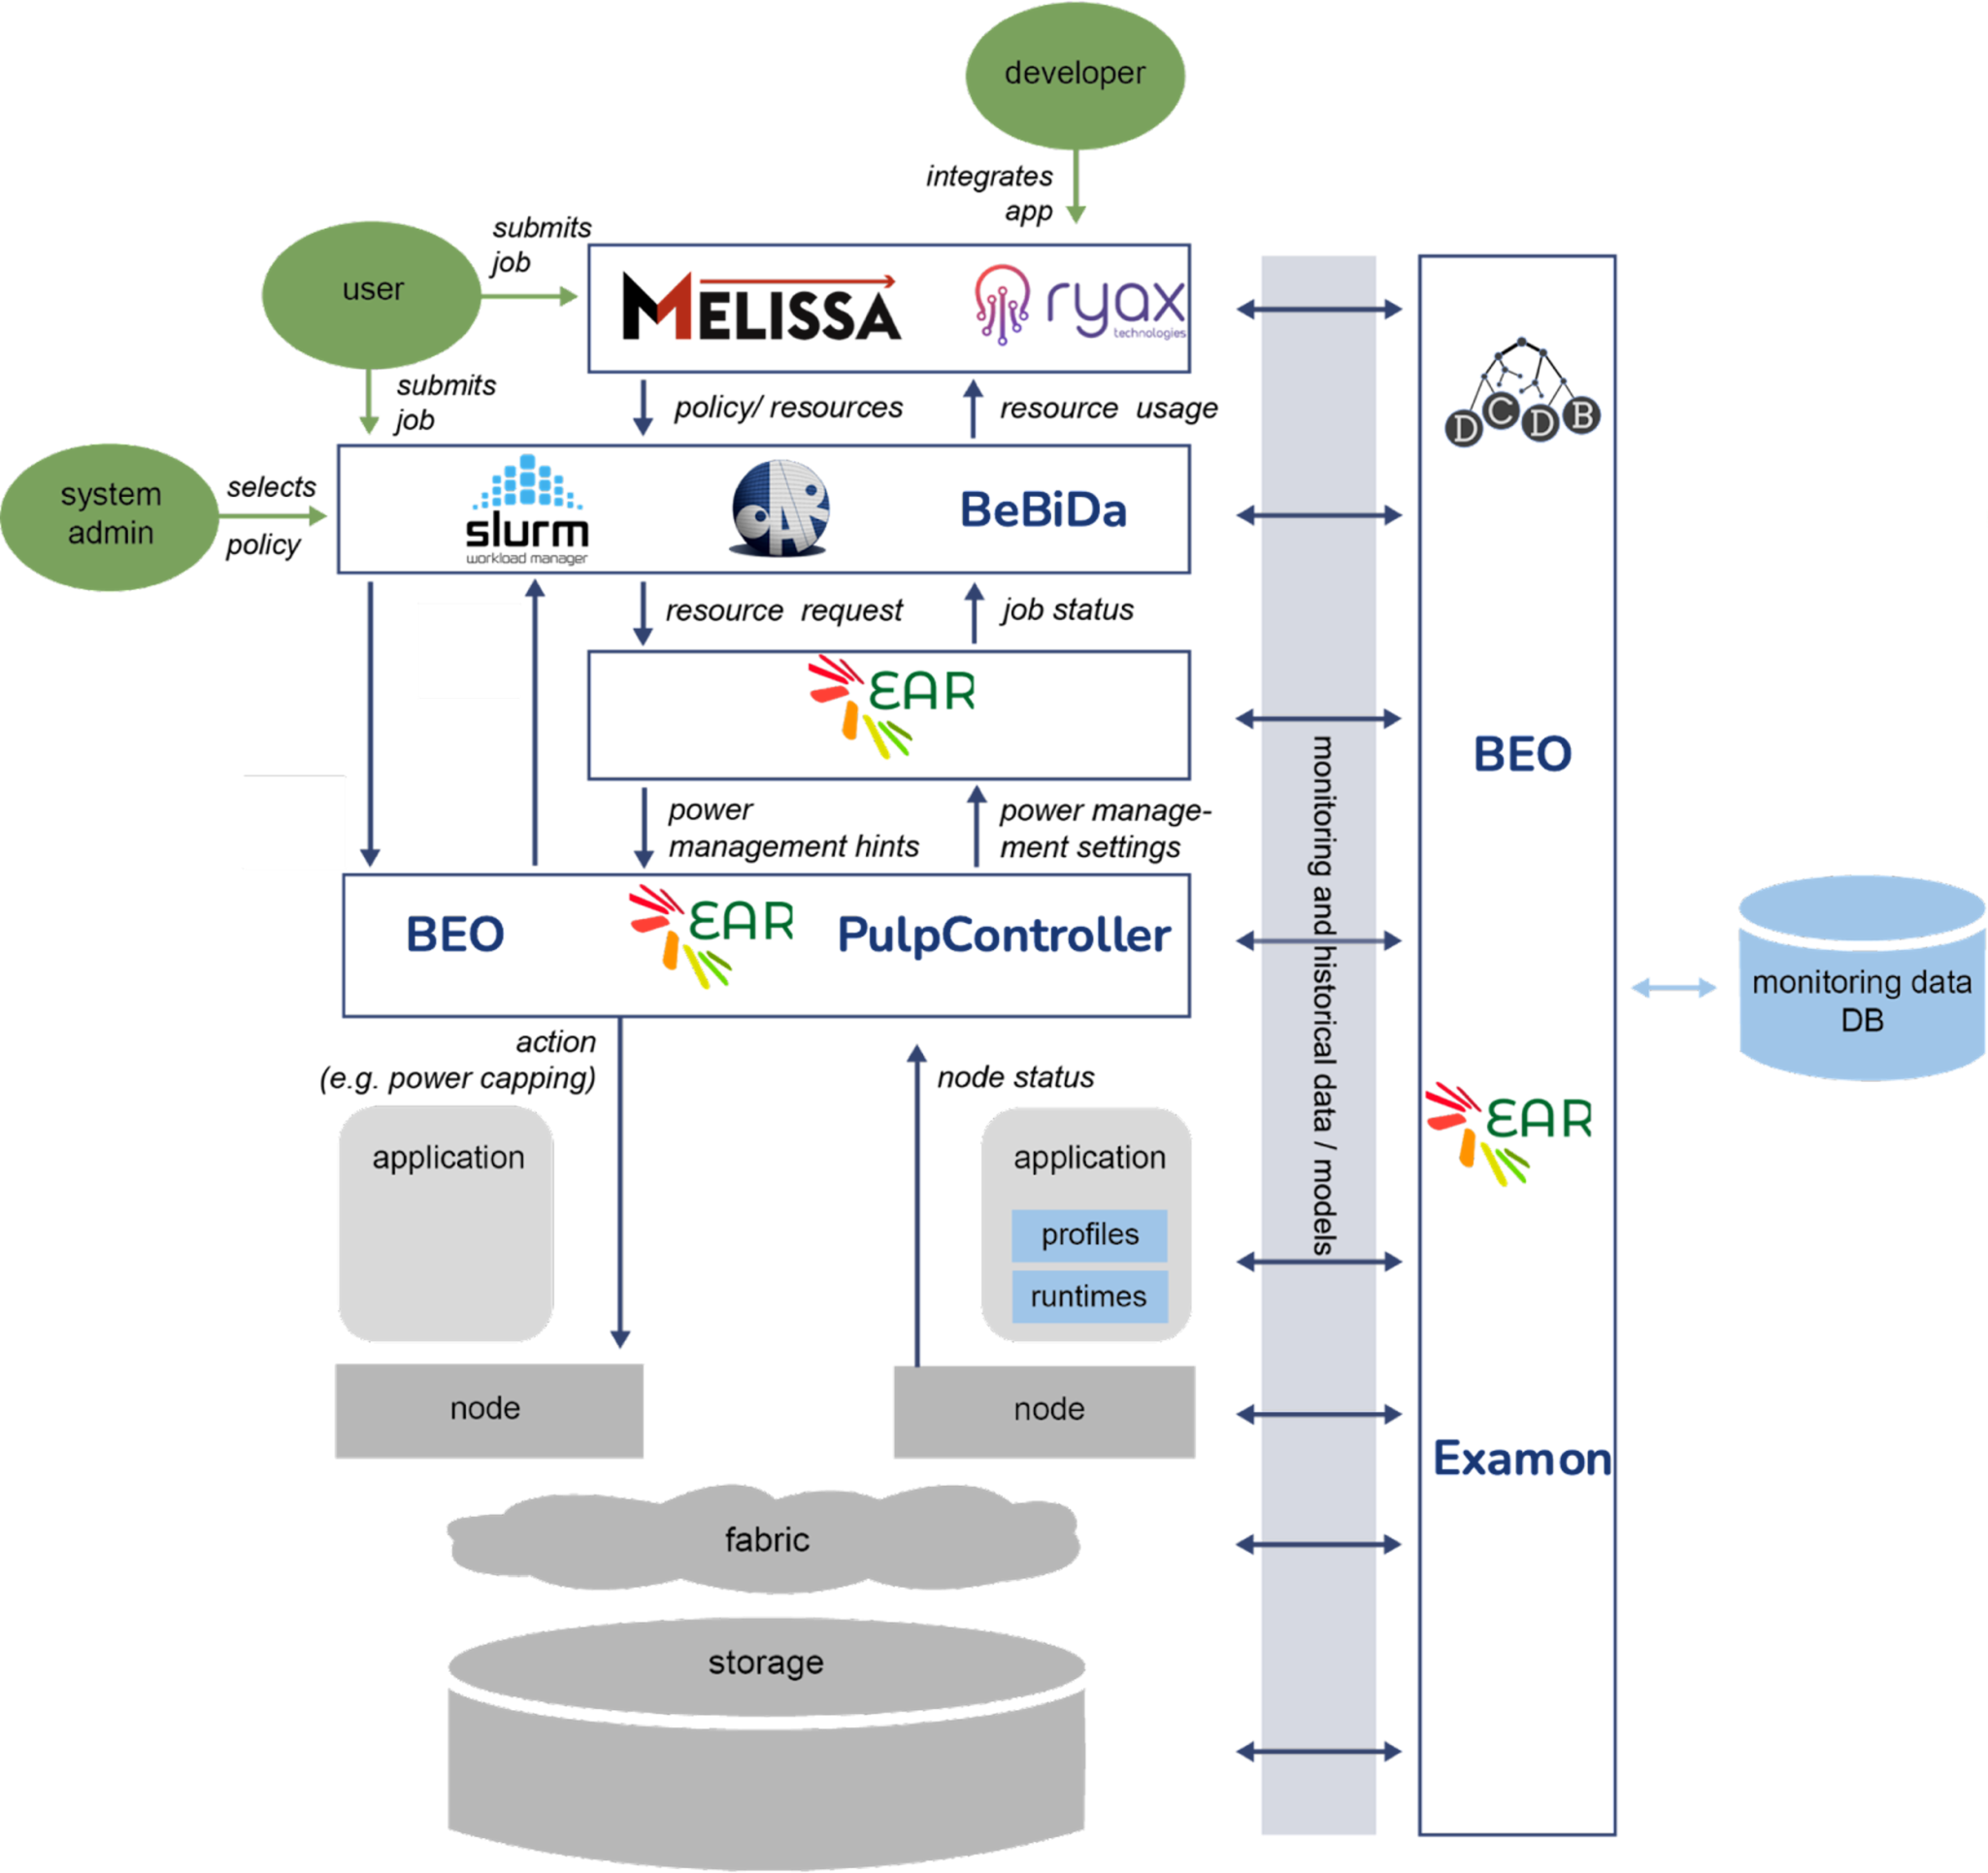
\includegraphics[width=\textwidth]{img/REGALE_USE.png}
    \caption{Copertura componenti}\label{fig:regale_cover}
    \end{subfigure}
    \caption{Implementazione dei componenti secondo il modello del Power stack}
\end{figure}

\section{Integrazione}
Vista la natura dei software introdotti nel progetto, non era previsto che questi potessero scambiare informazioni tra di loro, in quanto nati per essere usati singolarmente. Visto che creare versioni che permettesse agli attori del power stack di comunicare due a due non era conveniente, si è scelto di procedere con un \textbf{middleware DDS}. %Questa tesi è nata in collaborazione con REGALE, ed è stata stilata anche per riportare test utili alla finalità di REGALE.
\chapter{Test}
Il tema principale di questa tesi, è stata quelli di generare un modello, analizzare e alla fine implementare quello che potrebbe essere l'infrastruttura sulla quale tutti gli attori di un Power-Stack 
possano comunicare in modo completamente distribuito tramite DDS. Per poter creare l'infrastruttura necessaria, sono stati utilizzati sistemi di High-Performance Computing sui quali andare a provare empiricamente i vari esperimenti. Per supportare questo lavoro, sono stati resi disponibili due supercomputer uno da Cineca\cite{Cineca} e uno da E4\cite{E4} nel tentativo di ottenere risultati affidabili. Di seguito le specifiche dei sistemi utilizzati:
%In questo capitolo verranno riportati i casi studio e i test effettuati sul framework. %Tutti questi sono stati eseguiti su un sistema HPC Galielo-100 Cineca con le specifiche riportate nella tabella seguente

\begin{table}[H]
\begin{center}
    %TODO: Da riscrivere in italiano
\begin{tabular}{l|l|l}
    \hline
    \textbf{Parameter} & \textbf{Cineca} & \textbf{E4} \\
    \hline
    Number of nodes used & 3 & 3\\
    \hline
    Processor & Intel CascadeLake 8260 & Intel CascadeLake 8260  \\
    \hline
    Number of sockets per node & 2 \\
    \hline
    Number of cores per socket & 24 \\
    \hline
    Memory size per node & 384 GB \\
    \hline
    Interconnect & Mellanox Infiniband 100GbE \\
    \hline
    OS & CentOS Linux \\ 
    \hline
    MPI & Open MPI  4.1.1 \\
    \hline
\end{tabular}
\end{center}
\caption{Tabella hardware dei sistemi utilizzati}
\label{table:hpc-cineca}
\end{table}

% In tutti i test successivi, ove non specificato diversamente sono stati usati 1 publisher e 48 subscriber su diversi nodi. Questo è stato fatto per provare la scalabilità, visto che nel testbed che è stato utilizzato, erano presenti 48 core (1 core per ogni subscriber).

\section{Strumenti utilizzati}%Struttura dei test
I test effettuati in questa sezione sono stati generati da diversi tipi di componenti ognuno di essi con uno o più compiti specifici, in modo da avere un discreto controllo sull'avanzamento e la gestione dei dati. Nella figura \ref{fig:schema_global} viene riportato uno schema riassuntivo di tutte le tecnologie utilizzate.
\begin{figure}[H]
    \centering
    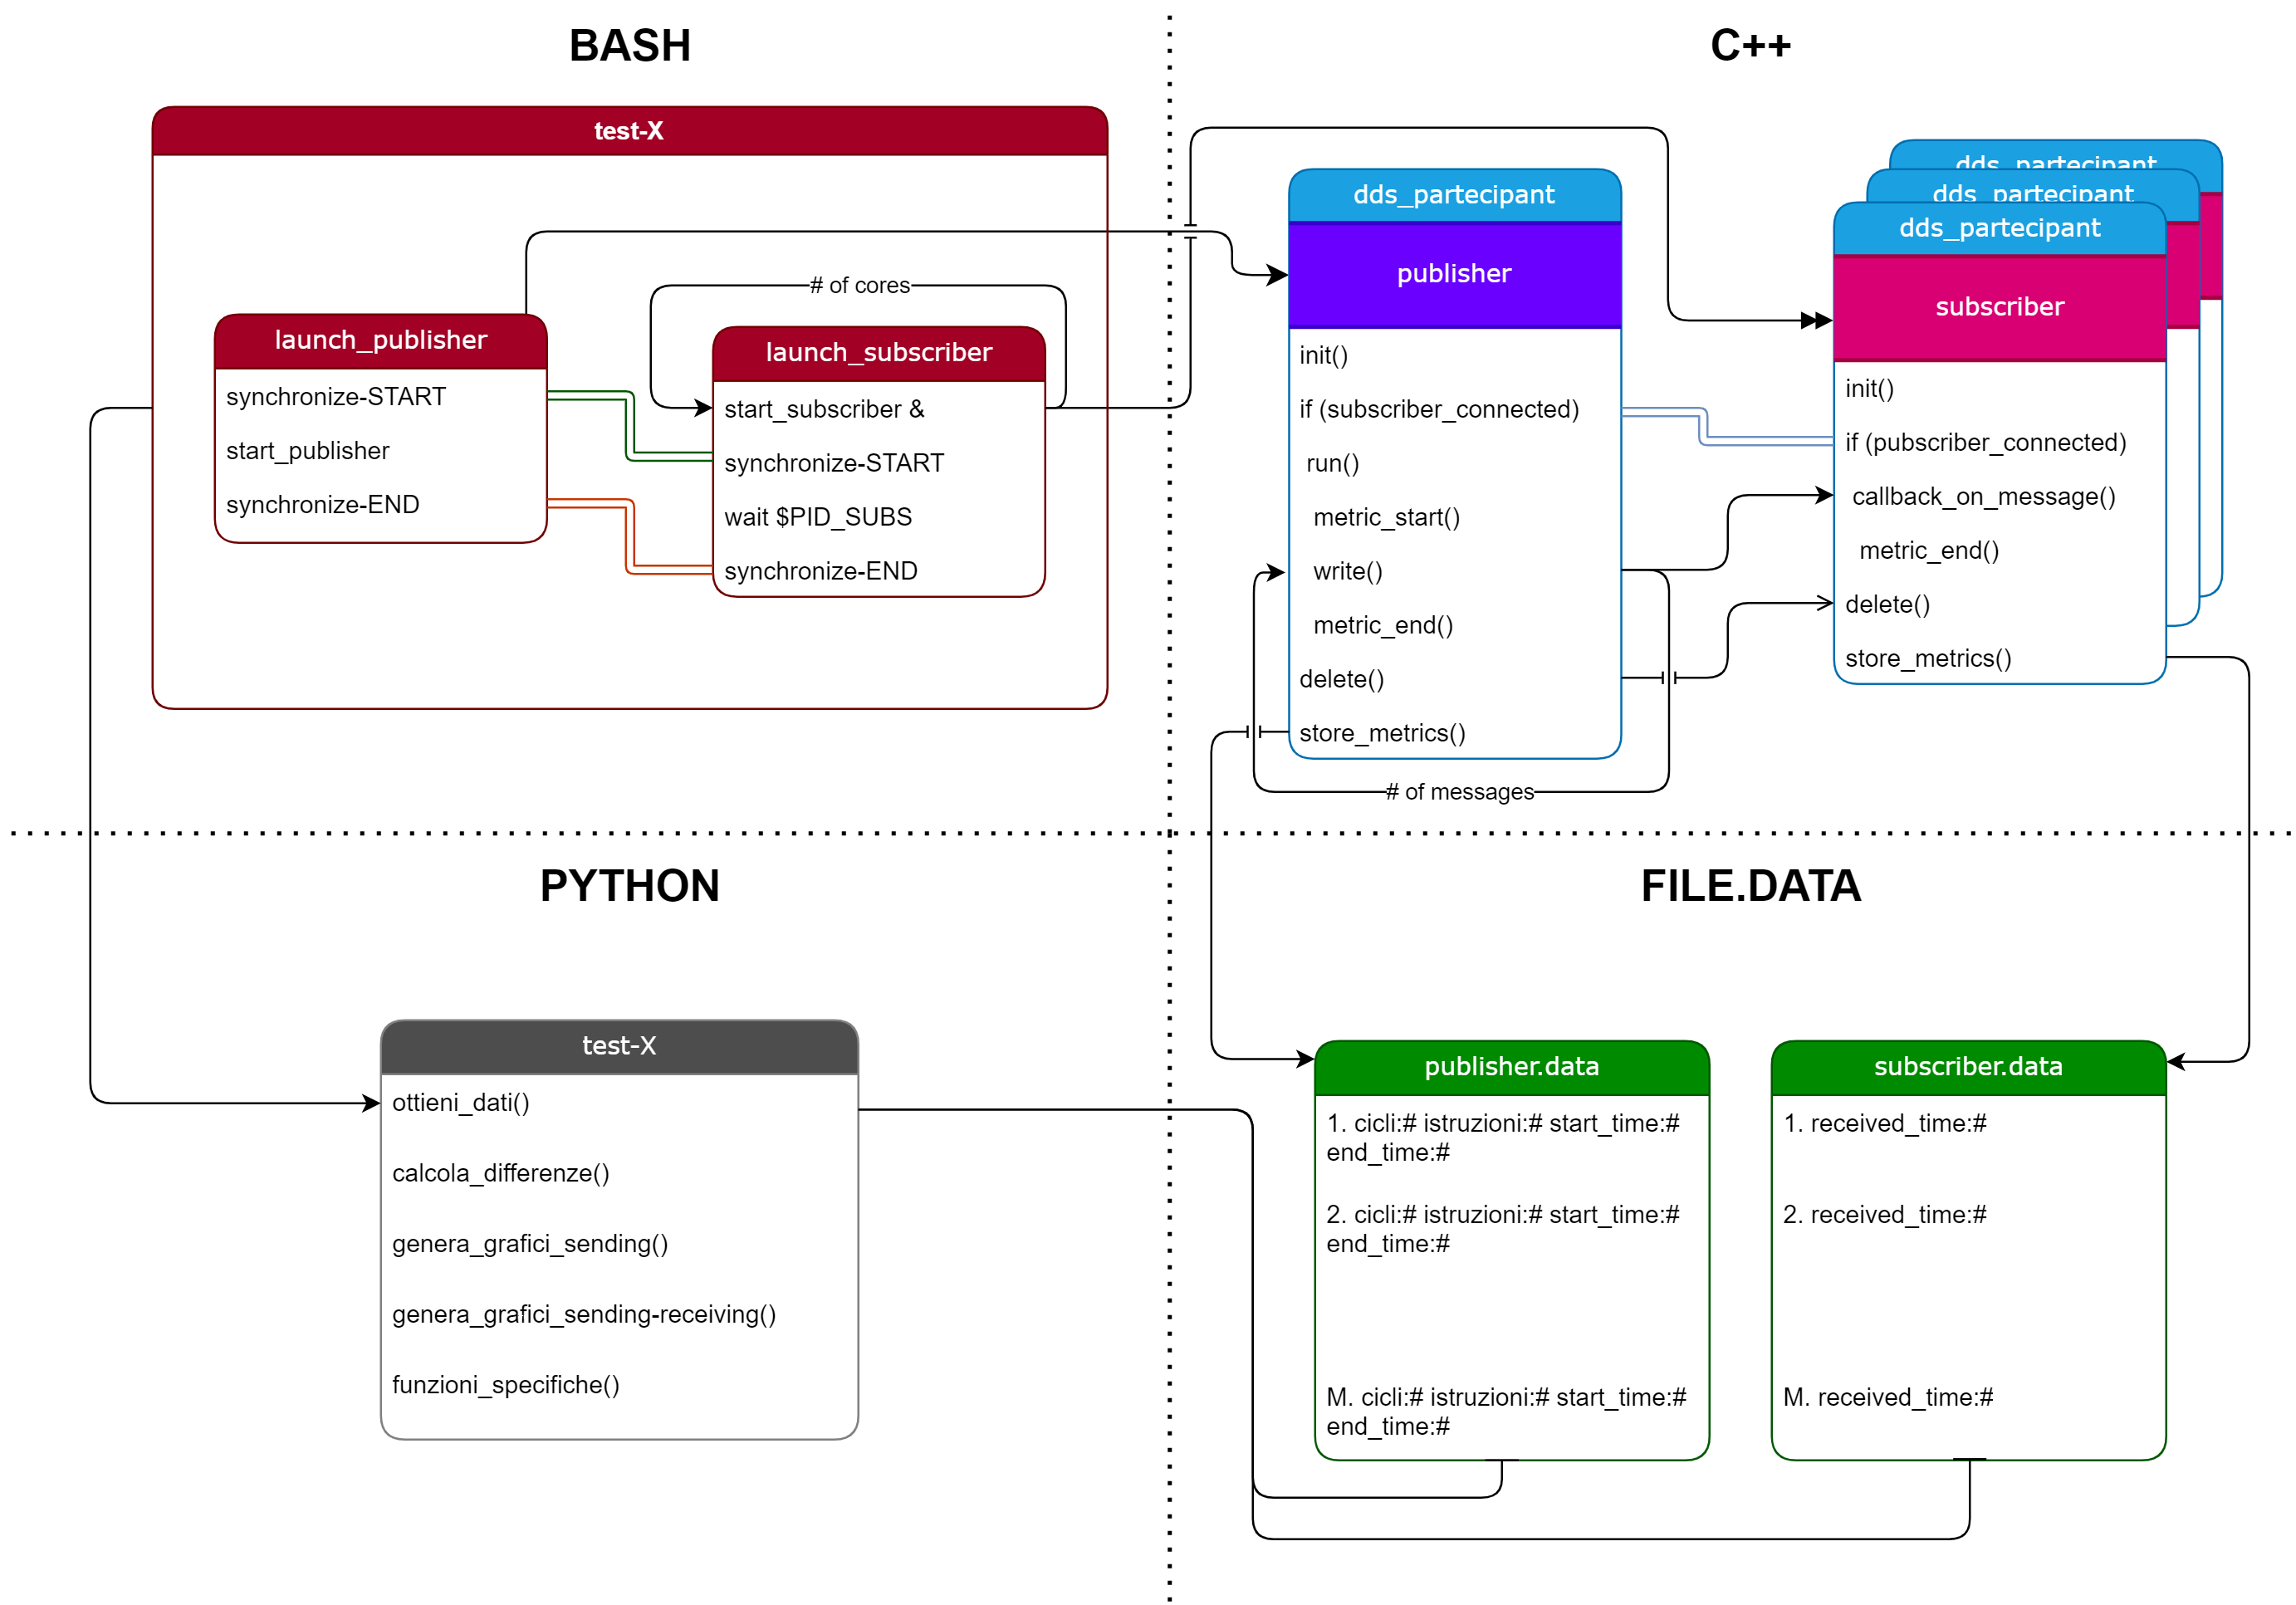
\includegraphics[width=\textwidth]{./img/schema_test_globale.drawio.png}
    \caption{Struttura test} %TODO: add readtsc, istr
    \label{fig:schema_global}
\end{figure}

\subsection{Bash}\label[Sezione]{sec:Shell}
Vista la necessità di lanciare diversi publisher e diversi subscriber ogni volta con dei parametri variabili è stato conveniente usare programmi di scripting come \gls{Bash}. Infatti questi gestivano i diversi parametri da passare agli attori, inizializzavano le variabili d'ambiente, decidevano quali core dovevano essere utilizzati da ogni partecipante (task-setaffinity) e mantenevano sincronizzati i test per evitare che alcuni attori fossero inizializzati troppo presto. Infine ripulivano e ordinavano i dati una volta terminato i test ed andavano ad eseguire gli script python che processavano i dati, nelle cartelle corrette.
\subsection{C++}

E' stato scelto di realizzare una unica implementazione publisher e subscriber dove i valore delle funzionalità che si volevano testare dovevano essere passati come parametro lato bash (\ref{sec:Shell}) in modo da poter avviare tutti i test con gli stessi codici, rendendo più semplice la gestione dei diversi test, e più robusto ad errori dovuti a diverse configurazioni.
\subsubsection*{Struttura}

Per scambiarsi dei messaggi all'interno di infrastruttura basata su DDS, sono necessari: (i) un topic, (ii)un publisher ed (iii) un subscriber. Inoltre nel topic è necessario definire il tipo dato o struttura di dati che si va a scambiare. La struttura che si è scelta di utilizzare per i test è stata la seguente:
\begin{verbatim}
    struct DDSTest
    {
        unsigned long index;
        std::string message;
    };
\end{verbatim}
Dove index era necessario per definire una corrispondenza stretta tra i messaggi inviati e quelli ricevuti, mentre la stringa era comoda per definire un oggetto di dimensione molto variabile (anche dinamicamente durante i test).

Una volta studiata la documentazione ufficiale di eProsima FastDDS, è stato sviluppato un codice in grado di integrare tutte le funzionalità di DDS ed alcuni strumenti per l'ottenimento di metriche precedentemente concordate con Cineca\cite{Cineca}. Nello specifico sono state scelte:
\begin{itemize}
    \item Tempo di invio
    \item Istruzioni Perf-Event per invio
    \item Cicli TSC (read\_tsc) per invio
    \item Tempo di invio e ricezione
\end{itemize}
\subsection{Lettura TSC}
Il Time Stamp Counter, è un registro a 64 bit, presente nella maggior parte dei processori moderni. Il registro fornisce informazioni sul tempo, in termini di cicli di clock del processore, e viene spesso utilizzato per effettuare misure di queste metriche. Per leggere questo valore, che viene fatto prima e dopo l'istruzione da misurare, è necessario eseguire la seguente istruzione:
\begin{verbatim}
    unsigned int lo, hi;
    __asm__ __volatile__ ("rdtsc" : "=a" (lo), "=d" (hi));
    return ((uint64_t)hi << 32) | lo; 
\end{verbatim}
\emph{rdtsc} è l'istruzione \gls{assembly} per leggere il registro Timestamp Counter, =a (lo) e =d (hi) sono i vincoli di output che specificano come i risultati dell'istruzione rdtsc devono essere restituiti al programma. In lo ("=a") viene riportat il valore a 32 bit meno significativo ed in hi, il valore a 32 bit più significativo.

\subsection{Conteggio istruzioni}
Per le istruzioni invece è stato usato lo strumento \textbf{Perf}, un software offerto da Linux ed incluso anche nel suo \gls{Kernel}, per la profilazione delle performance tramite i \emph{performance\_counter}. Questa suite è estremamente avanzata e permette di ottenere delle metriche specifiche senza troppa difficolta. In questo caso è stata usata una chiamata alla libreria \textbf{perf\_event} nel codice per il valore \emph{PERF\_COUNT\_HW\_INSTRUCTIONS}.

\subsection{Ottenimento dei tempi}
In sistemi molto complessi come può essere considerato un supercalcolatore, la gestione degli orologi è tutt'altro che banale. Infatti dopo aver deciso una tra le tante politiche di sincronizzazione disponibile come centralizzata, distribuita, GPS e tante altre, è necessario applicarle e continuare a tenere questi orologi sullo stesso tempo assoluto. Nei sistemi utilizzati in questo progetto, ed in particolare nei sistemi \ref{table:hpc-cineca}, lo strumento adottato è Network Time Protocol (fornito da \gls{Ntpd}). Quest'utlimo ogni intervallo di tempo impostato, va a rendere disponibile ai vari nodi ed ai rispettivi orologi locali un tempo di riferimento che ha la funzione di punto fisso. Questo intervallo è normalmente fissato ogni 1024s, ma non disponendo dei diritti necessari ad utilizzarlo, non mi è stato possibile recuperare l'informazione.

Detto questo, per ottenere le differenze di tempi su sistemi Linux, è ricorrente utilizzare una funzione chiamata \textbf{clock\_gettime()} che restituisce il tempo istantaneo alla chiamata. Se si esegue la differenza tra due diverse clock\_gettime(), si ottiene il tempo trascorso tra queste due.
Per questa funzione è possibile ottenere diverse metriche tra cui:
\begin{itemize}
    \item CLOCK\_REALTIME: ottiene il tempo assoluto, sincronizzato dei vari sistemi da ntpd
    \item CLOCK\_MONOTONIC: ottiene un tempo relativo, da un punto non preciso dall'avvio del sistema
    \item CLOCK\_MONOTONIC\_RAW: come sopra, ma non influenzato da ntpd
    \item CLOCK\_PROCESS\_CPUTIME\_ID: timer dei processori ad alta risoluzione
    \item CLOCK\_THREAD\_CPUTIME\_ID: tempo dei thread dei processori
\end{itemize}
Tra queste è stato utilizzato il MONOTONIC, visto che il REALTIME con aggiornamenti di ntpd di 1024s subisce variazioni di alcuni millisecondi\cite{ntpd}, di gran lunga superiore all'ordine di grandezza da misurare (microsecondi, a volte anche nanosecondi). Inoltre dato che per eseguire i test è stato usato un solo sistema per volta (o Cineca, o E4) MONOTONIC\_RAW non era necessario (anche in caso di aggiornamento ntp, viene diffuso in egual modo su tutti i nodi).
Il problema di usare la MONOTONIC, è che su sistemi con orologi diversi, questi sono sfasati di diverse migliaia di secondi. E' stato necessario aggirare questo problema, e per farlo sono stati usati 2 approcci completamente diversi:
\begin{itemize}
    \item Sincronizzazione dei nodi
    \item RTT
\end{itemize} 

\noindent Entrambi i tentativi verranno approfonditi nelle successive sezioni \ref{TODO}


\subsubsection{UML}
Lo schema UML di funzionamento degli attori DDS è riassunto e schematizzato dalla figura \ref{fig:uml}
\begin{figure}[H]
    \centering
    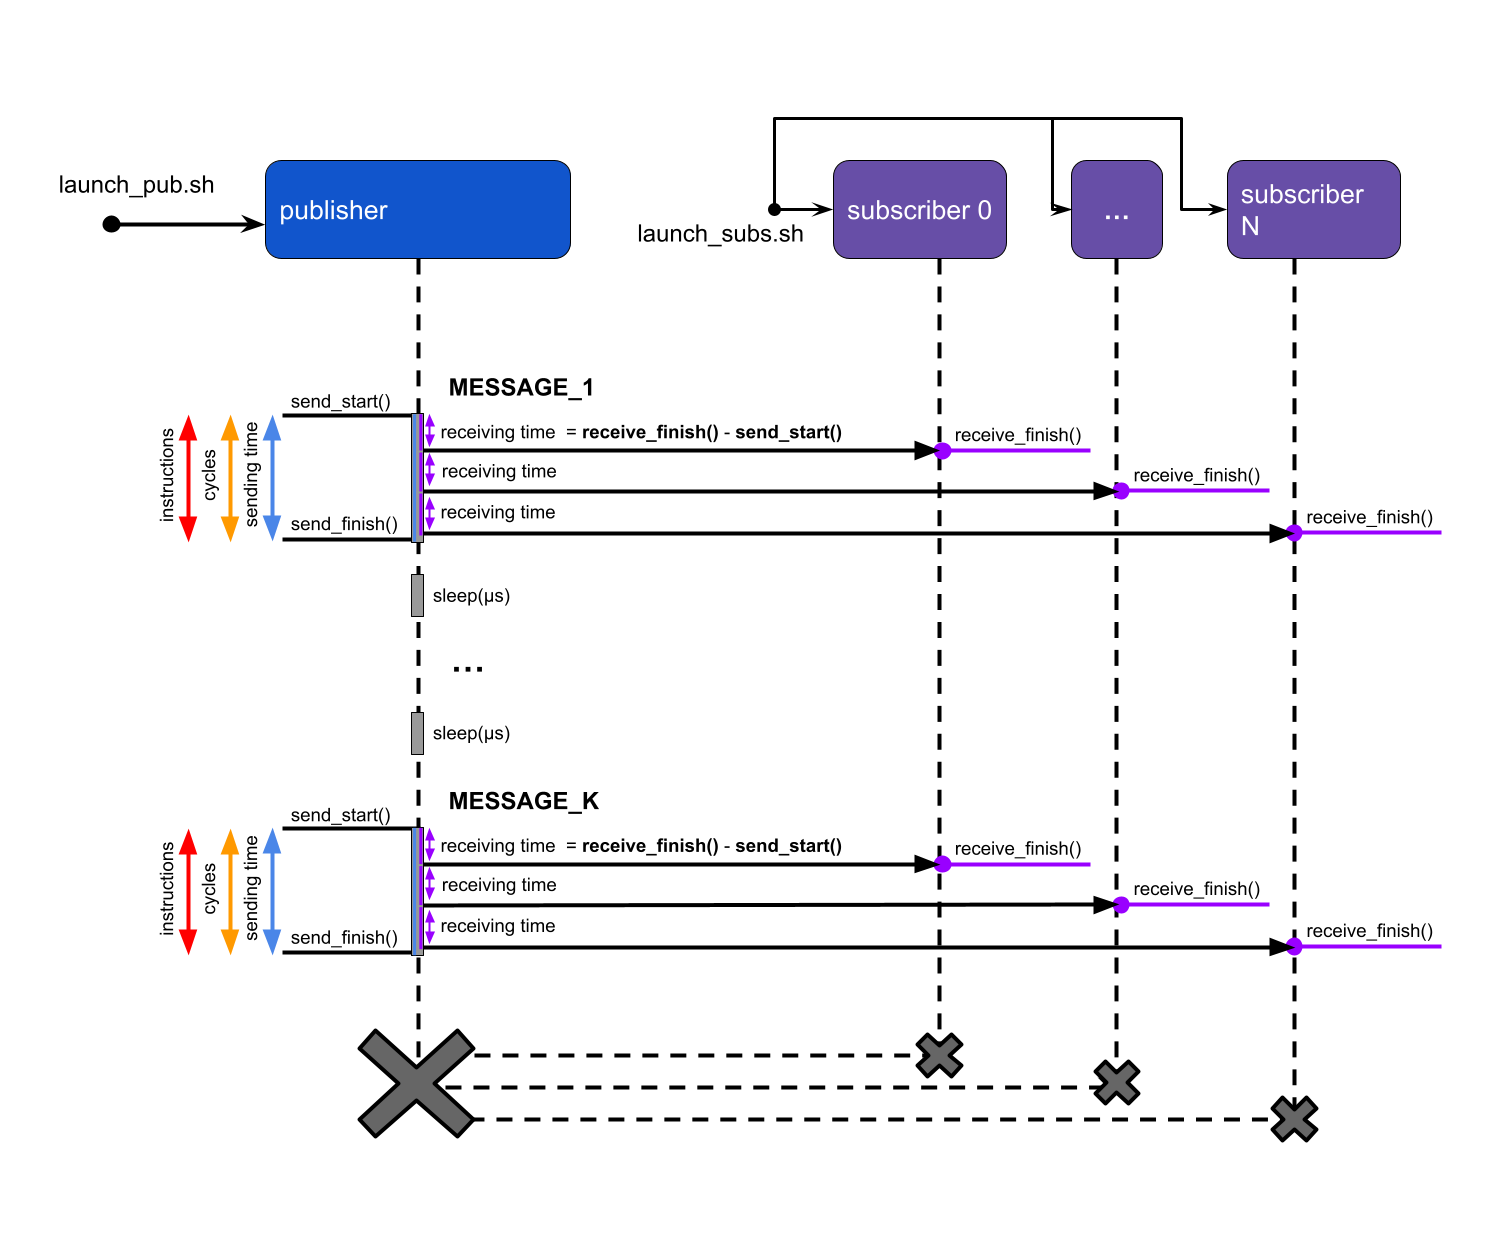
\includegraphics[width=\textwidth]{./img/umel-send-receive.png}
    \caption{Schema UML} %TODO: typo on receiving time = recIVE
    \label{fig:uml}
\end{figure}

In particolare nel Publisher \ref{actor:publisher} prima e dopo la chiamata a funzione di write() %TODO: inserire nella tesi?
si sono presi i valori tempo-invio, istruzioni, e TSC, mentre al lato ricevente, di Subscriber \ref{actor:subscriber} è stato preso il tempo al momento dell'arrivo del messaggio. Segue uno schema uml della base di ognuno dei test.

%TODO: se serve approfondire TSC, e metriche eseguite prima e dopo

\section{DataMiners}
Considerando che ogni publisher genera 10 mila messaggi da inviare a tutti e 48 i subscriber, per ogni protocollo di trasporto, e in alcuni casi in partizioni differenti si è arrivato ad avere per ogni test fino a $1'960'000$ messaggi scambiati e le relative metriche per ogni messaggio da processare. 
Gli script python sono stati utili a organizzare e processare tutti i dati prodotti dai vari test. Inoltre sono stati fondamentali per poter generare tutti i grafici che sono stati in questa tesi.

\section{Sincronizzazione}\label{sec:timesync}
Una delle prime soluzioni che è stata provata, è stata quella di sincronizzare gli orologi locali dei diversi nodi tramite l'utilizzo di librerie sviluppate per la programmazione parallela come Message Passing Interface (MPI). Quest'ultimo è un protocollo di comunicazione molto utilizzato nei sistemi HPC per la programmazione parallela.
Nello specifico è stata utilizzata una funzionalità chiamata MPI\_barrier, che permette di bloccare i processi, fino all'arrivo di un punto in comune, dopo il quale tutti procedono insieme. Questo serve per sincronizzare i processi tra di loro, ma non è ideata nello specifico per sincronizzare gli orologi. Gli strumenti strumenti utili alla mera sincronizzazione dei tempi dei nodi sono altri, come il già citato Network Time Protocol,
ma essendo ntpd un servizio di amministrazioni non è stato possibile interagirci e quindi usarli. Nella figure \ref{fig:sync_time_shift1} \ref{fig:sync_time_shift2} \ref{fig:sync_time_shift3} sono stati riportati i dati ottenuti grazie a questo meccanismo.

\begin{figure}[H]
    \centering
    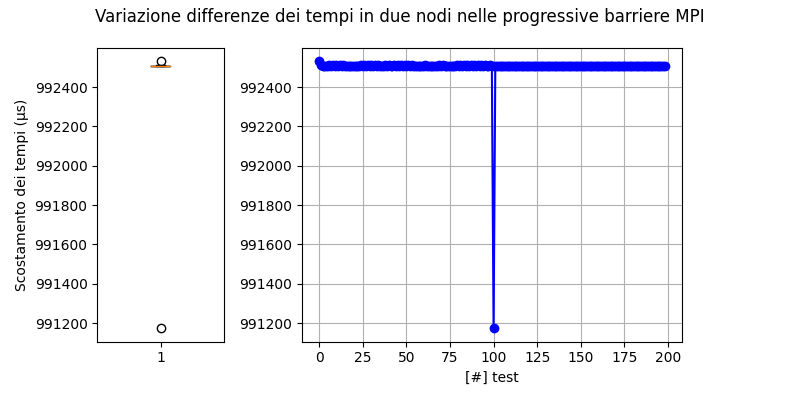
\includegraphics[width=\textwidth]{./results/time_sync_node.png}
    \caption{Scostamento del tempo su nodi diversi}
    \label{fig:sync_time_shift1}
\end{figure}
\begin{figure}[H]
    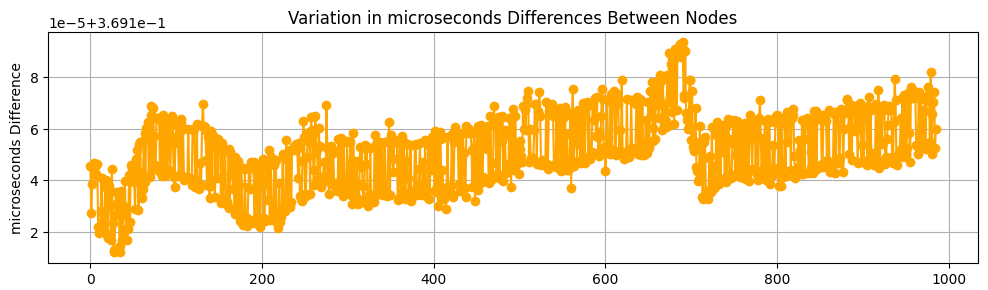
\includegraphics[width=0.99\textwidth]{./results/time_shift_clean.png}
    \caption{Scostamento senza outliers}
    \label{fig:sync_diff_distr2}
\end{figure}
\begin{figure}[H]
    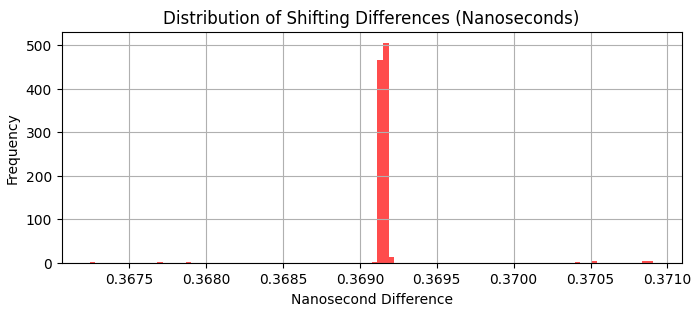
\includegraphics[width=\textwidth]{./results/time_sync_distribution.png}
    \caption{Distribuzione delle differenze}
    \label{fig:sync_diff_distr3}
\end{figure}

Come possibile notare nella figura \ref{fig:sync_time_shift1} nonostante le mpi\_barrier, gli scostamenti di tempo tra 2 nodi durante i diversi tentativi effettuati (1000), cambia notevolmente, arrivando a differenze fino ad un massimo di 290 microsecondi. Questo rende il metodo appena mostrato utilizzabile solo nel caso in cui non sia necessario sapere il tempo assoluto di qualche azione, ma le varianze, che rimarrebbero costanti se si utilizzano sempre gli stessi nodi.


\section{RTT}\label{sec:timeRTT}
Nonostante la sincronizzazione, fosse idealmente il metodo più preciso per ottenere i tempi di invio-rivezione, essendo l'errore possibile dello stesso ordine di grandezza dei tempi di ricezione, per alcuni test si è utilizzato un approccio che non richiedesse sincronizzazione. Il metodo più intuitivo è utilizzare il Round Trip Time (RTT).
Il RTT è un metrica che viene solitamente utilizzata per misurare la latenza di una rete, e si basa sull'idea di calcolare il tempo che intercorre tra lìinvio di un segnale e la ricezione della conferma di arrivo dello stesso. Ovviamente il valore ottenuto risulta nel caso ideale più che raddoppiato vista la necessità di un messaggio di risposta. Nel diagramma \ref{fig:uml} non sarebbe stato possibile condurre questa misura, perchè un subscriber non può inviare un messaggio di risposta.
Per farlo è stato necessario rivedere gli attori coinvolti, ed introdurre in quello che prima venivano chiamati publisher e subscriber, un publisher e un subscriber a testa.
Per semplificarne la comprensione viene riportato lo schema modificato:

\begin{figure}[H]
    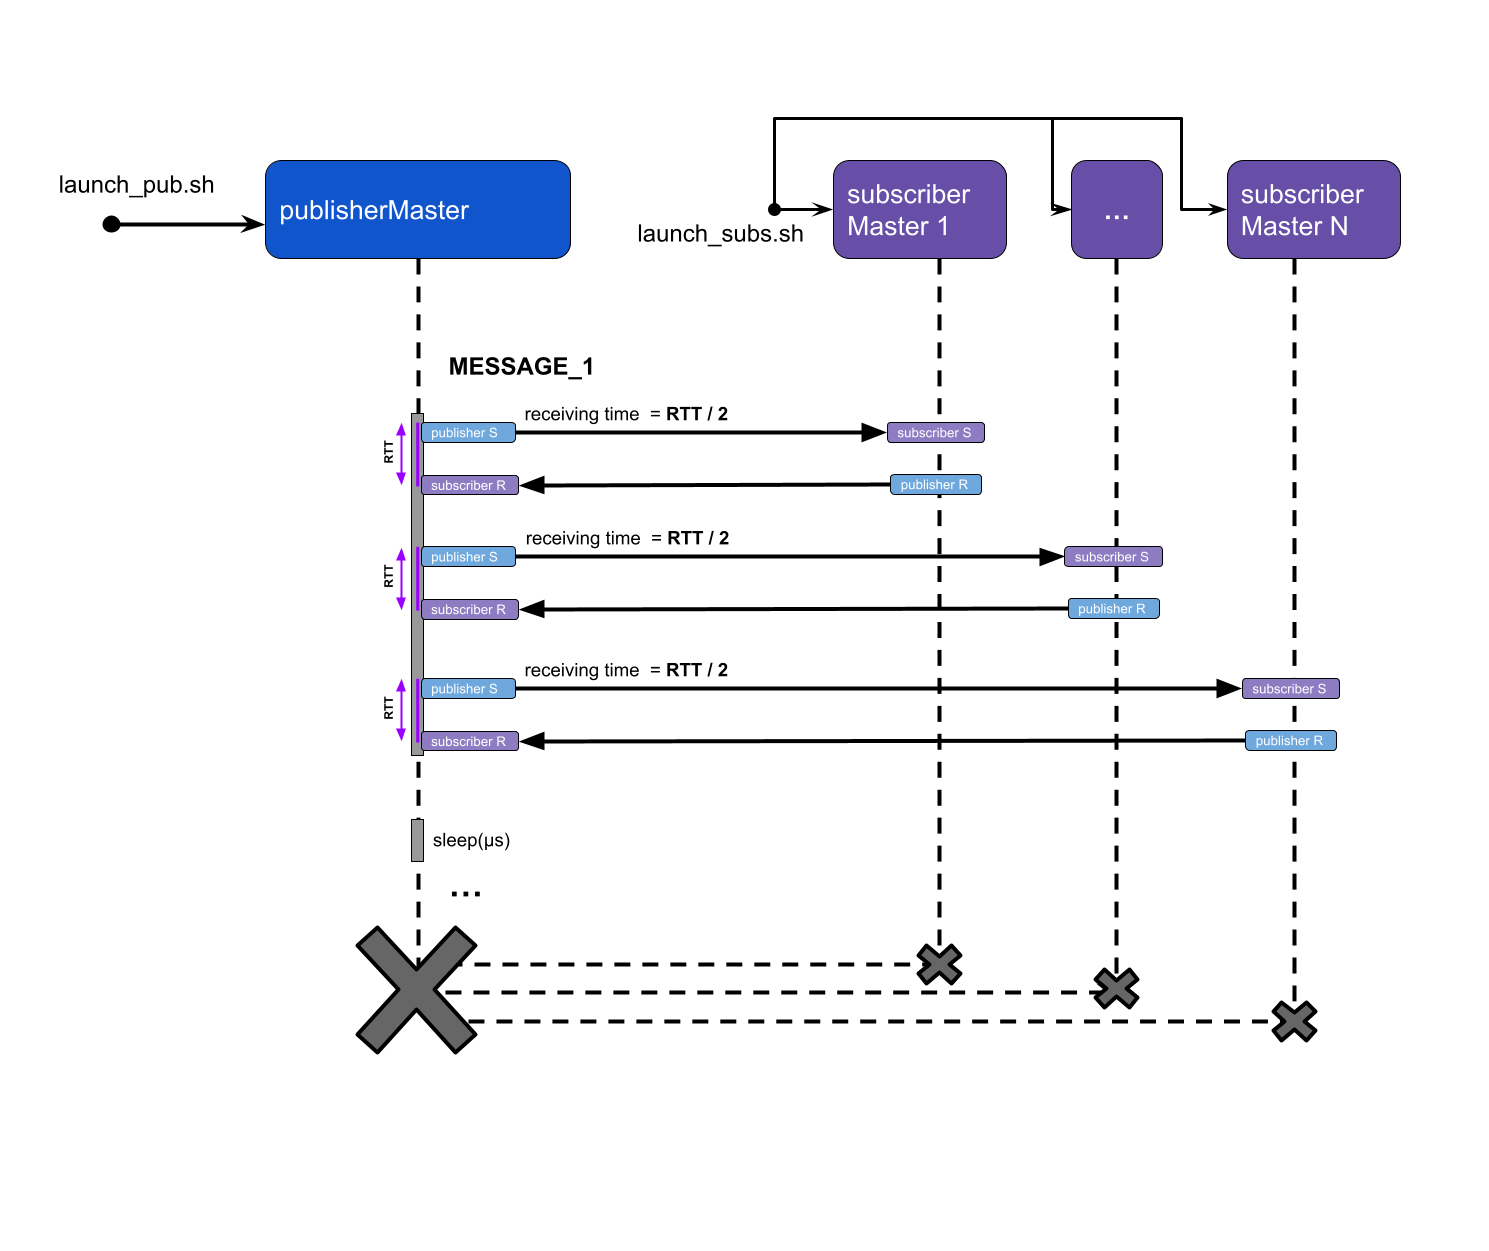
\includegraphics[width=\textwidth]{./img/RTT.png}
    \caption{Schema UML RTT}
    \label{fig:rtt_uml}
\end{figure} 

Ovviamente questo metodo può comportare qualche ritardo intrinseco di dover gestire due entità per ogni attore, ma sono tempi infinitesimali in confronto al tempo necessario per inviare il messaggio su rete (dove è stato usato questo approccio).

\section{Schema}
Sono stati svolti diversi test al fine di trovare un modello ottimale di utilizzo e per la caratterizzazione di DDS, all'interno di sitemi HPC, nel contesto del Power Management. Nello specifico i test sono stati utili a capire il peso che avesse una singola configurazione o modello di utilizzo al fine di trovare quello più adeguato per una futura implementazione. I test effettuati sono:

\begin{itemize}
    \item test-0: discovery
    \item test-1: protocollo di comunicazione
    \item test-2: partizioni e wildcards
    \item test-3: throughput
\end{itemize}


Al fine di condurli nel modo più trasparente e corretto possibile sono stati resi pubblici \cite{mygit} tutti i codici utilizzati durante lo svolgimento di questi test. %TODO5O: riordinare & documentare git


\subsection{Test-0}
La prima fase di DDS consiste nel riconoscere altri \emph{dds-partecipant} appartenenti allo stesso dominio. Questa viene chiamata \textbf{fase di Discovery}. Essa ha un ruolo estremamente importante siccome senza non sarebbe possibile far comunicare nessun attore all'interno della stessa rete e nemmeno nello stesso nodo. Una delle peculiarità di DDS è che permette di eseguire tutto in modo completamente distribuito, e anche questa fase non viene fatta diversamente (se non esplicitamente configurato). Il problema è che durante la discovery, quando si hanno diverse migliaia di componenti, si genera un overhead di pacchetti scambiati e di conseguenza anche le computazioni necessarie che crescono esponenzialmente. %Ovviamente la natura effimera di alcuni di questi componenti potrebbe aggravare il problema. 
Sono disponibili in DDS, anche per questo motivo, meccanismi di discovery centralizzati al fine di evitare questo problema. In questo esperimento si andranno a comparare le due diverse implementazioni e per farlo si userà \textbf{perf}.
%CONTROLLA CHE SI POSSA FARE TCPDUMP SU CINECA

\subsection{Test-1}
In DDS ed in particolare nel layer sottostante di RTPS, per scambiare messaggi anche tramite rete, e non solo nello stesso nodo, è possibile scegliere come mezzo diversi tipi di protocolli:

\begin{itemize}
    \item udp: fornisce due versioni v4 e v6 e importa l'omonimo protocollo di trasporto
    \item tcp: fornisce due versioni v4 e v6 e importa l'omonimo protocollo di trasporto
    \item udp-multicast: una versione modificata del semplice udp, dove tutti i subscriber collegati allo stesso topic, hanno un indirizzo comune di ricezione dei dati, permettendo così al publisher di inviare un singolo messaggio che viene condiviso tra tutti i subscriber  % TODO: uml
    \item shared-memory: analogo al metodo precedentemente, ma invece di utilizzare un indirizzo IP, viene utilizzato un indirizzo di memoria. E' possibile solo quando i due processi che comunicano sono sullo stesso nodo, con memoria condivisa.
\end{itemize}

Nel primo test si è valutata la differenza di queste implementazioni utilizzando la rete infiniband \ref{table:hpc} su diversi nodi di un supercalcolatore. 

\subsection{Test-2}
Un concetto fondamentale nelle comunicazioni tra attori con gerarchie diverse, in sistemi con diverse centinaia di migliaia di entita, come cluster, nodi, processori, workflow, job (etc.), sono le possibilità di instradare, segmentare e rendere gerarchiche le comunicazioni. Come spiegatolo nel capitolo \ref{Chapter:dds} in DDS ci sono diversi strumenti disponibili per farlo. Tra di loro differiscono per alcuni aspetti, come flessibilità, costo (in performance) e livello di segmentazione.

\subsubsection*{Dominio} 
Il dominio è la segmentazione di più "forte" e di più alto livello. Va a partizionare gli attori presenti in un dominio in modo del tutto fisico (cambiando per ogni dominio porte e indirizzi di comunicazione) e per nulla flessibile. Per cambiare il dominio è necessario distruggere e creare di nuovo il partecipante. Inoltre il dominio non permette nessun tipo di gerarchia.
    
\subsubsection*{Topic}
All'interno di un dominio i topic definiscono il metodo principale di instradamento dei messaggi, essendo però limitato dal tipo di messaggio che si vuole inviare. Infatti topic diversi supportano tipi di dato diversi, e non sono modificabili a run-time. %TODO: glossario
Inoltre il topic non permette gerarchie ed è difficilmente modificabile a run-time

\subsubsection*{Partizione}
Questo strumento risulta molto interessante, in quanto all'interno di un topic permette di definire gerarchie (è possibile sottoscriversi a più partizioni contemporaneamente), definisce wildcards e crea una segmentazione virtuale. Inoltre è facilmente modificabile a run-time.

\subsubsection{Wildcards}
Le wildcards sono un costrutto appartenente alle partizioni, che permette di definire dei pattern testuali sulla base del quale vengono instradati i messaggi. Un esempio può essere \textit{Node*} che va a corrisponde a tutti i messaggi sotto il topic precedentemente definito, a tutte le partizioni che iniziano con Node.

\begin{figure}[H]
    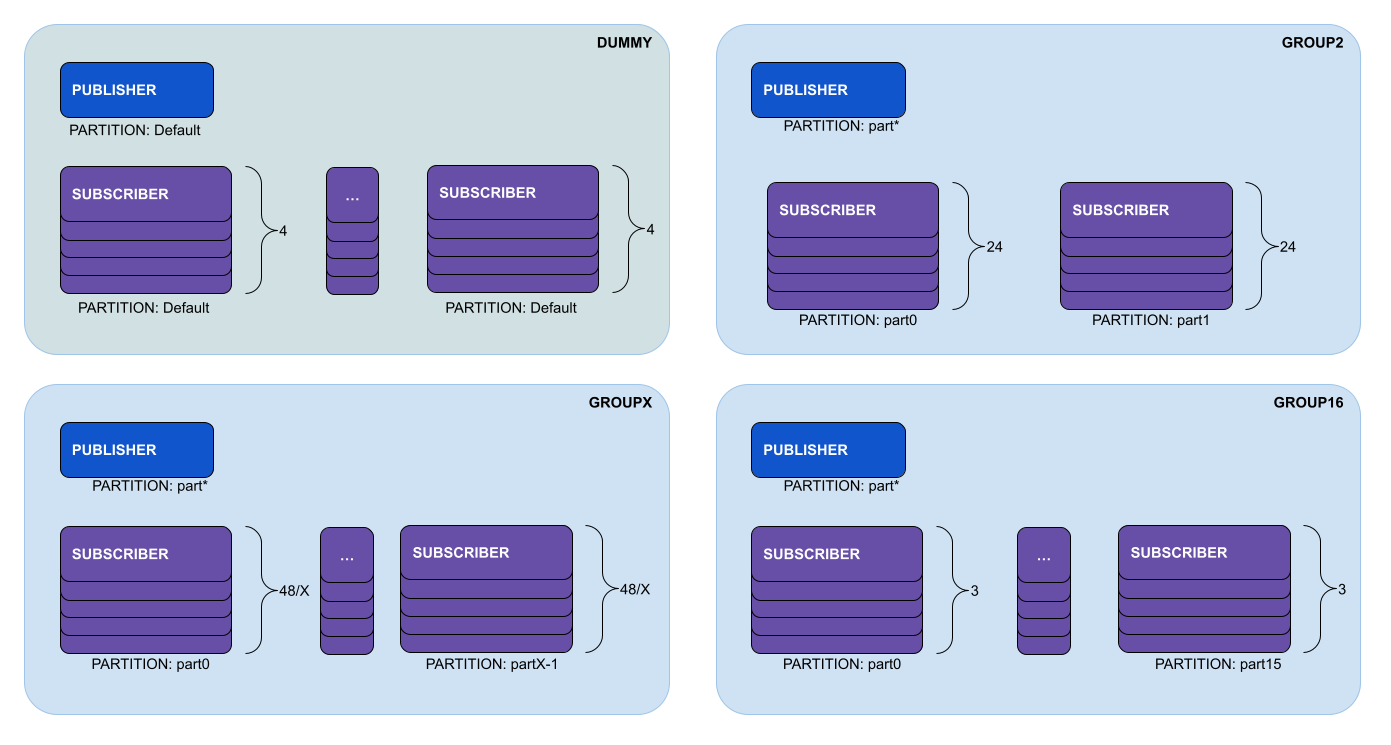
\includegraphics[width=\textwidth]{./img/wildcards.png}
    \caption{Schema test wildcards}
    \label{fig:test_UML_wildcards}
\end{figure} 


%In questo test si è valutata la differenza in termini di performance dei diversi strumenti, con un particolare focus sulle partizioni e le wildcards rese disponibili in esso.
Definiti questi concetti è stato pensato un test rappresentato dalla figura \ref{fig:test_UML_wildcards} per valutare se utilizzare la partizioni, e quindi sfruttare le gerarchie negli instradamenti avesse un prezzo in termini di performance da pagare.  


\subsection{Test-3}
Nel l'ultimo test si è è voluto ottenere dei valori rappresentativi della teconologia studiata. In particolare si sono visti valori come il throughput e la bandwidth massima per ciascun protocollo.
Per calcolarlo sono stati scelte configurazioni che potessero simulare un carico di comunicazioni elevato tra attori di HPC. Nella tabella \ref{table:test3} vengono riportate i parametri scelti.

\begin{table}[H]
    \begin{center}
    \begin{tabular}{l|l}
        \hline
        \textbf{Parametri} & \textbf{Valore}\\
        \hline
        [\#] publisher & 1 \\
        \hline
        [\#] subscriber & 40 \\
        \hline
        [\#] messaggi scambiati (per attore) & 10 000 \\
        \hline
        Dimensione del messaggio & 16 Byte \\
        \hline
    \end{tabular}
    \end{center}
    \caption{Valori usati per il test 3}\label{table:test3}
    \end{table}
    

\chapter{Risultati}%Caratterizzazione DDS su HPC
% Visti i diversi risultati si può dire che è meglio usare i topic per* le partizioni per *
% etc etc

Nella sezione corrente, vengono riportati tutti i risultati rilevanti ottenuti durante la fase di testing stilando, dove possibile, un modello di utilizzo utile alle finalità di Power Management.
\section{Discovery: centralizzata vs distribuita}
Come previsto, nella fase di discovery un numero elevato di entità genera una quantità di di pacchetti scambiati che cresce in modo esponenziale. In questo caso sono stati usati tutti i core di due nodi, con un totale di 96 entità.
Già nel primo grafico~\ref{fig:test0pack}, con il numero di pacchetti sull'asse Y e il numero di entita sull'asse X, è possibile notare un distacco tra i due approcci, con sole 30 unità. Nella figura~\ref{fig:test0cicl} con i cicli sulle Y, numero entità sulle X, e nella figura~\ref{fig:test0_instr} con istruzioni sulle Y, viene confermato l'andamento non lineare.
%TODO change 90s graph
\begin{figure}[H]
    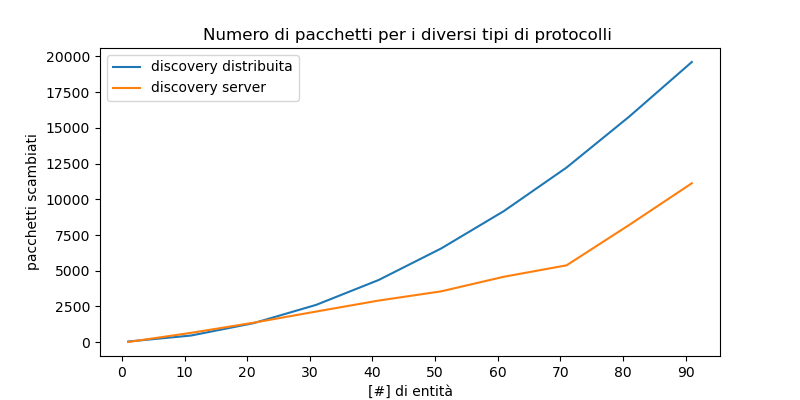
\includegraphics[width=\textwidth]{./results/test0_packet.png} 
    \caption{Numero di pacchetti scambiati durante la discovery all'aumentare di entità}\label{fig:test0pack}
\end{figure}
\begin{figure}[H]
    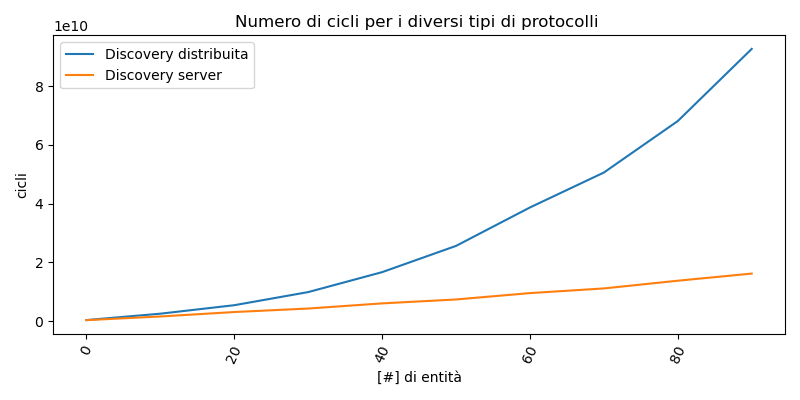
\includegraphics[width=\textwidth]{./results/test0_cicli.png} 
    \caption{Numero di cicli durante la discovery all'aumentare di entità nelle diverse opzioni}\label{fig:test0cicl}
\end{figure}
\begin{figure}[H]
    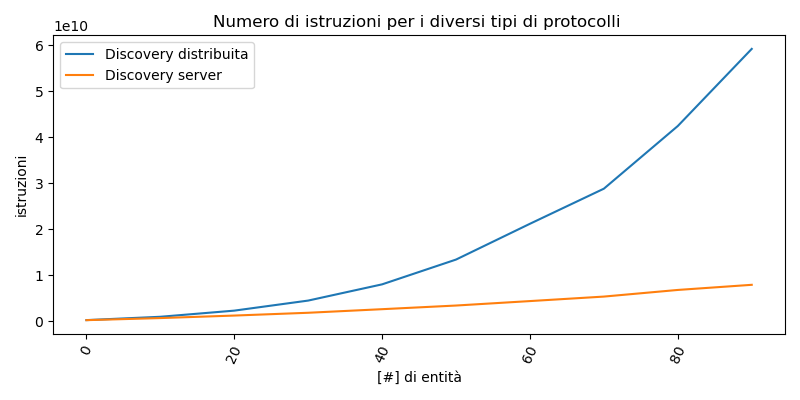
\includegraphics[width=\textwidth]{./results/test0_istruzioni.png} 
    \caption{Numero di cicli durante la discovery all'aumentare di entità nelle diverse opzioni}\label{fig:test0_instr}
\end{figure}
In un caso reale serve valutare in primo luogo il numero di entità in un determinato dominio, e successivamente i costi-benefici di ogni implementazione considerando anche l'impatto che si può avere nel caso di fallimento del server (nonostante sia possibile avere un server di backup che viene automaticamente attivato, nel caso il primo fallisse).

\section{Scalabilità del numero di subscriber iscritti ad un topic}
Visto lo schema~\ref{fig:uml} si può capire, che il numero di subscriber presenti in un dominio ed iscritti ad un topic, comporta un overhead di comunicazione che va ad influenzare sia i tempi, che cicli e istruzioni impiegate nella singola \emph{publish}. Questo viene dimostrato nella figura~\ref{fig:test3_overhead} (con i tempi medi di invio sulle Y) e~\ref{fig:test3_latenza} (con latenza media di ricezione in asse Y). In tutte le figure sull'asse X viene riportato il numero di subscriber che cresce fino a 40. L'effetto visto è particolarmente pronunciato anche in protocolli come \emph{UDP} che non possiedono concetti di connessione. Questo potrebbe essere dovuto al costo di inizializzazione ed invio dei messaggi, ad indirizzi di rete diversi.
\begin{figure}[H]
    \centering
    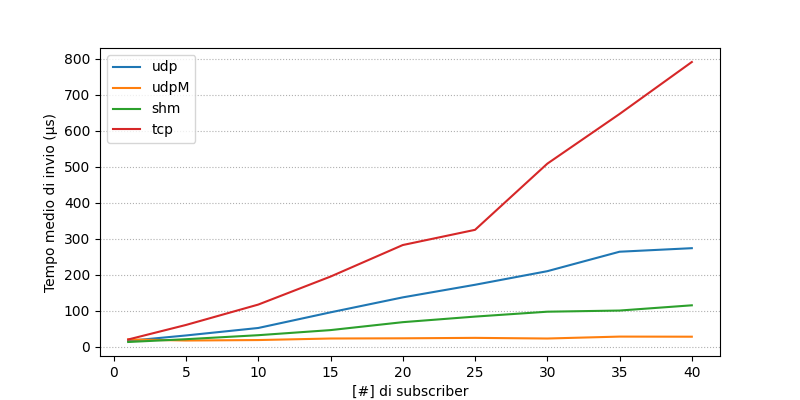
\includegraphics[width=\textwidth]{./results/test3_sending_multiplesub.png} %TODO, manca il titolo
    \caption{overhead sulla publish all'aumentare dei subscriber}\label{fig:test3_overhead}
\end{figure}
\begin{figure}[H]
    \centering
    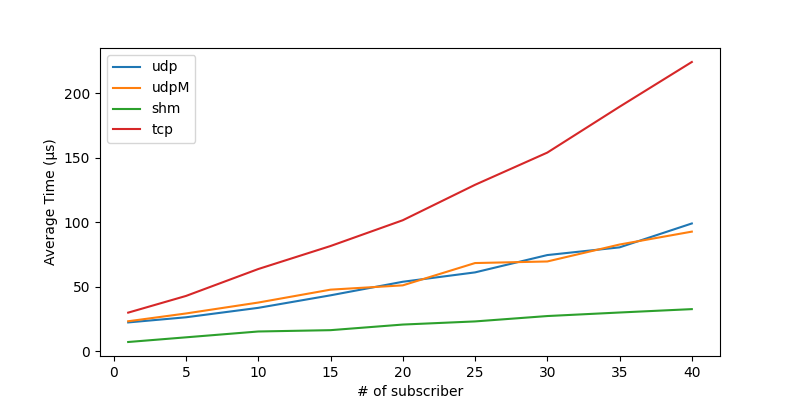
\includegraphics[width=\textwidth]{./results/test3_sendingreceiving_multiplesub.png} 
    \caption{latenza di ricezione all'aumentare dei subscriber}\label{fig:test3_latenza}
\end{figure}

Ovviamente l'impatto è poco significativo in quei protocolli che applicano strutture di multicasting come udp-Multicast e Shared-Memory, che verranno 

\begin{figure}[H]
        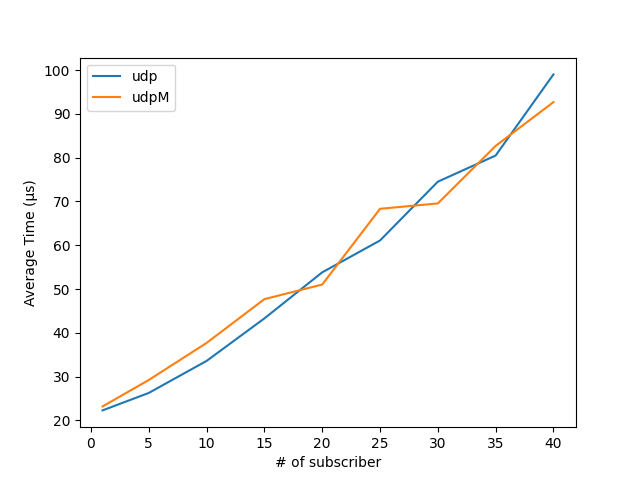
\includegraphics[width=\textwidth]{./results/test3_udpvsudpM.png} 
        \caption{Tempo di invio di un messaggio a [\#] subscriber nei protocolli UDP e UDP Multicast}\label{fig:udpvsudpMfigure}
\end{figure}

Da questo si può concludere che sia il publisher che subscriber risentono della presenza di molteplici \emph{dds-partecipant} in ascolto su un topic. Questo problema è migliorato nel caso vengano utilizzati protocolli che si basano su multicast. 

\section{Overhead sul primo messaggio}
E' stato notato con tutti i protocolli utilizzati un ritardo, di un ordine di grandezza superiore, che riguarda esclusivamente il primo messaggio. Tuttavia, non è stato chiarito il motivo di questo overhead, presente anche in comunicazioni locali\footnote{comunicazioni effettuati in localhost o in shared memory}. Anche se non dimostrato una delle possibili motivazioni potrebbe essere la necessità di allocare memoria durante la prima fase di comunicazione, da entrambi gli attori (potenzialmente amplificato nel caso~\ref{fig:rtt_uml}). In figura~\ref{fig:overhead_primo_messaggio} dove sugli assi Y viene mostrato il tempo di ricezione in microsecondi, e sull'asse X la sequenza dei messaggi, viene mostrato il problema citato.
\begin{figure}[H]
    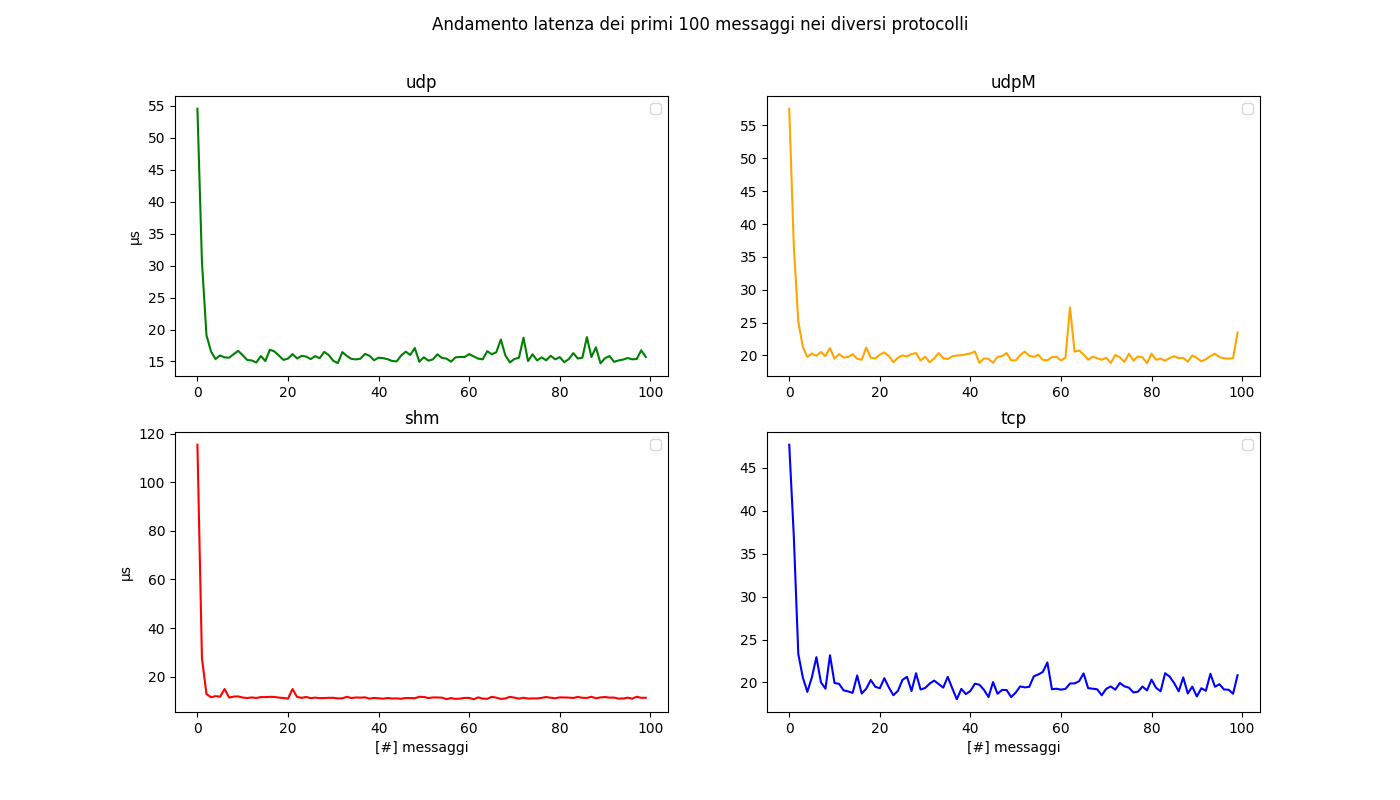
\includegraphics[width=\textwidth]{./results/errortest.png} 
    \caption{Overhead del primo messaggio nei vari protocolli}
    \label{fig:overhead_primo_messaggio}
\end{figure}
Infine, vista la mancanza di approfondimento verso tale problema, non si può concludere che l'invio di pochi messaggi sia sfavorito in questa implementazione.

\section{Protocolli di comunicazione}
Visti gli schemi~\ref{fig:minpowerstackscheme} è risulta probabile che in un Power Stack, siano predilette le comunicazioni non locali. In merito a ciò, nonostante ci siano di mezzo molti più livelli per comunicare con udp e tcp, i risultati trovati sono stati decisamente interessanti e non così lontani dal più veloce \emph{Shared Memory}. 
In figura~\ref{fig:test3_different_protocols} sugli assi X il numero di subscriber, e sulle Y le latenza di ricezione in microsecondi.
\begin{figure}[H]
    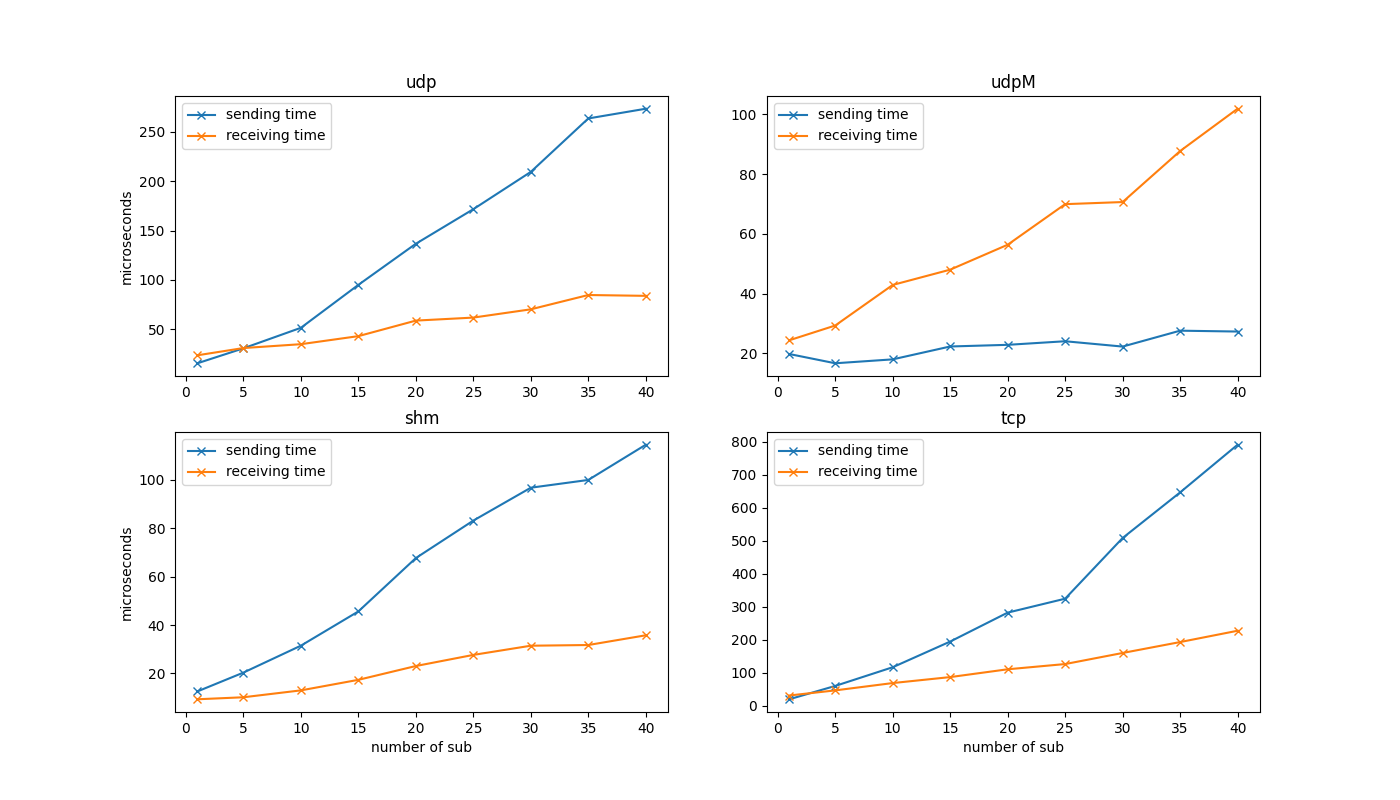
\includegraphics[width=\textwidth]{./results/test3_different_protocol_send_receive.png} 
        \caption{differenza della latenza di ricezione dei vari protocolli con }\label{fig:test3_different_protocols}
\end{figure}
Invece, in figura~\ref{fig:test3_different_protocols2} e figura~\ref{fig:test1sdbox} sugli assi X i protocolli, mentre sulle Y per il primo solo le latenza di ricezione in microsecondi, e nel secondo sia latenza di ricezione che overhead di invio.
\begin{figure}[H]
    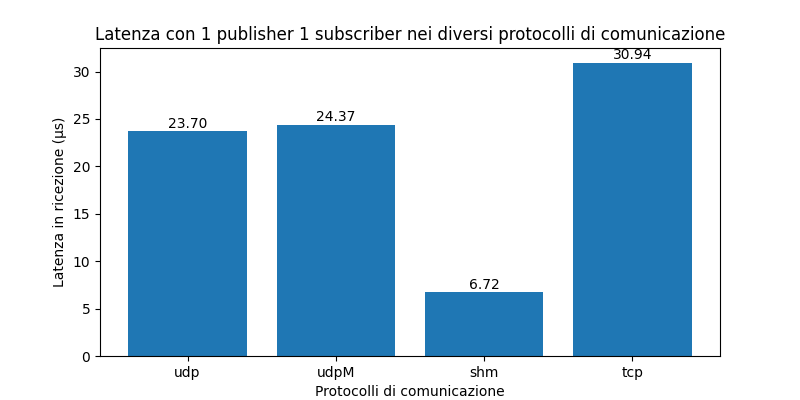
\includegraphics[width=\textwidth]{./results/test1_bar_sr_1p1s.png} 
        \caption{latenza media di ricezione di un singolo messaggio nei vari protocolli}\label{fig:test3_different_protocols2}%TODO Da sistemare protocol non va bene, label sbagliate etc
\end{figure}

\begin{figure}[H] %TODO: do this graph also for wildcards
    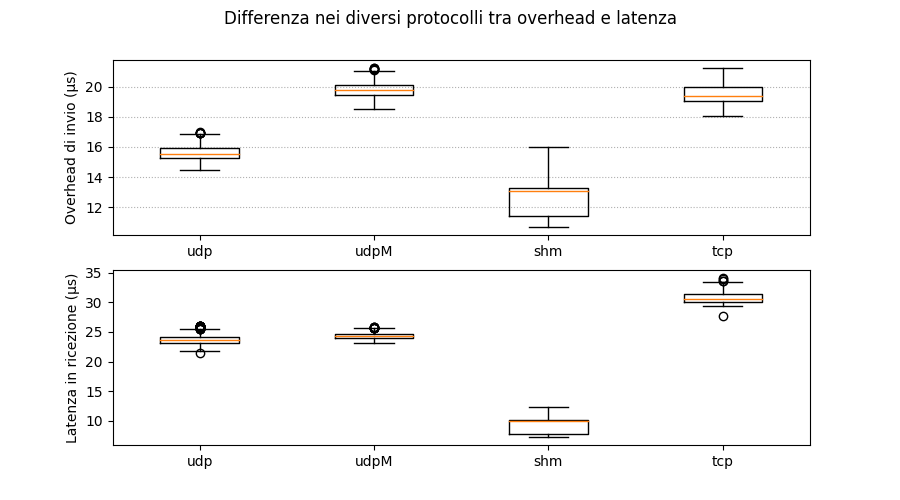
\includegraphics[width=\textwidth]{./results/test1_box_sr_1p1s.png} 
        \caption{diagramma a scatola nei vari protocolli di comunicazione con un publisher e un subscriber}\label{fig:test1sdbox}
\end{figure}
Infine, in figura~\ref{fig:test3_cycle_different_protocols} sugli assi X i protocolli, mentre sulle Y il conteggio di cicli e istruzioni ($10^6$).
\begin{figure}[H]
    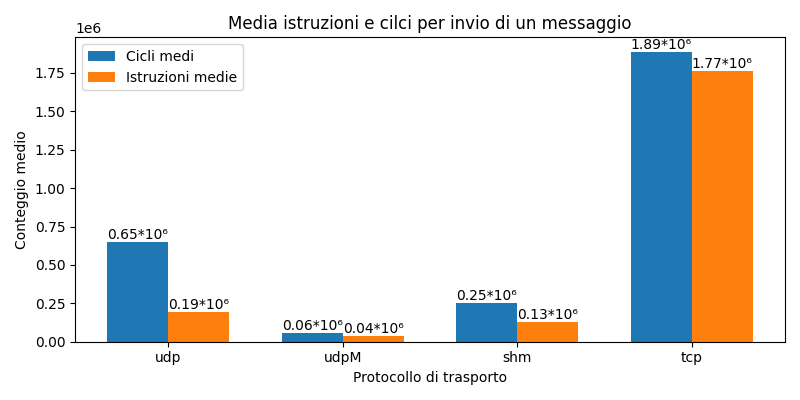
\includegraphics[width=\textwidth]{./results/test1_cyclinstr.png} 
        \caption{Conteggio cicli e istruzioni per ogni protocollo}\label{fig:test3_cycle_different_protocols}%TODO label overfull boxes
\end{figure}
E' quindi preferibile, ove possibile, usare \emph{Shared Memory} sia per prestazioni, che per evitare di saturare la rete. In secondo luogo, se in presenza di diversi subscriber, per non caricare il publisher usare \emph{UDP Multicast}. E infine utilizzare \emph{TCP} solo dove vi è necessità di connessione, visto le notevoli latenze si in scrittura che in lettura. In tutti gli altri casi, dove non si è in locale, e dove il numero di subscriber non supera qualche decina, risulta più che adeguato \emph{UDP}.

\section{Domini, Partizioni e Wildcards}
Nei test effettuati con topic e partizioni, non sono state notate differenze degne di nota in termini di performance nell'usare uno strumento piuttosto che un altro (\ref{fig:test2parttopicdomain}). Lo sono stati invece tra questi ultimi e i Domini. Tuttavia i domini non offrono alcun tipo di flessibilità e richiede il riavvio dei \emph{dds-partecipant} nel caso si necessiti di un qualsiasi cambiamento. Per questo è consigliato utilizzo di domini diversi, solo tra entità che non hanno necessità di comunicare, e che anzi, magari anche per motivi di sicurezza devono stare isolati. 
In figura~\ref{fig:test2parttopicdomain} sugli assi X il numero crescente di subscriber, e sulle Y conteggio medio di cicli ($10^6$).

\begin{figure}[H]
    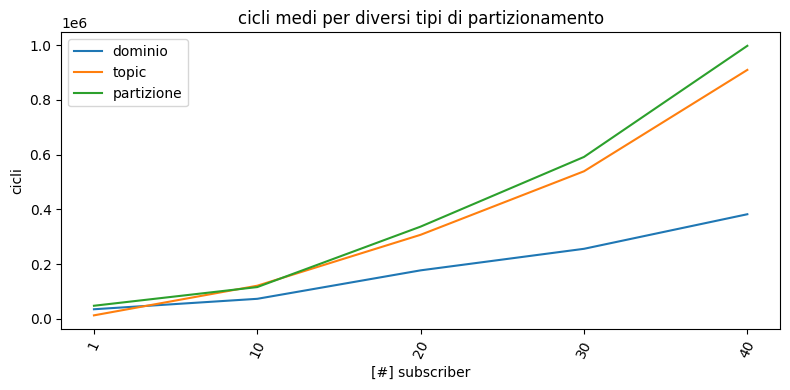
\includegraphics[width=\textwidth]{./results/test2_cicli_partvstopicvsdomaain.png} 
        \caption{Peso in termini di cicli nell'usare partizioni topic e domini}\label{fig:test2parttopicdomain}
\end{figure}

Per quanto riguarda entità che necessitano di gerarchie, è conveniente usare le partizioni con le Wildcards visto che non hanno un peso significativo come notabile in~\ref{fig:test2wildcards} dove sull'asse X vi è il numero di partizioni usate, mentre sulle Y il tempo di invio. Infine lasciando i topic come mezzo di partizionamento, per il tipo di dati, e il tipo di istruzioni da utilizzare.

\begin{figure}[H]
    \centering
    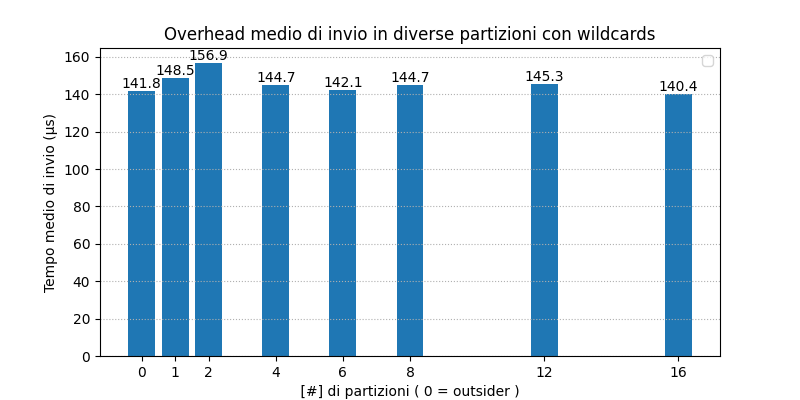
\includegraphics[width=\textwidth]{./results/test2_wildcards.png}

    \caption{Differenza in tempi di invio con utilizzo di wildcards in diverse partizioni}\label{fig:test2wildcards}
\end{figure}
Nella figura \ref{fig:test2cicl} sulle Y il conteggio di istruzioni e cicli ($10^6$) rispetto al numero di partizioni (sulle X).
\begin{figure}[H]
    \centering
    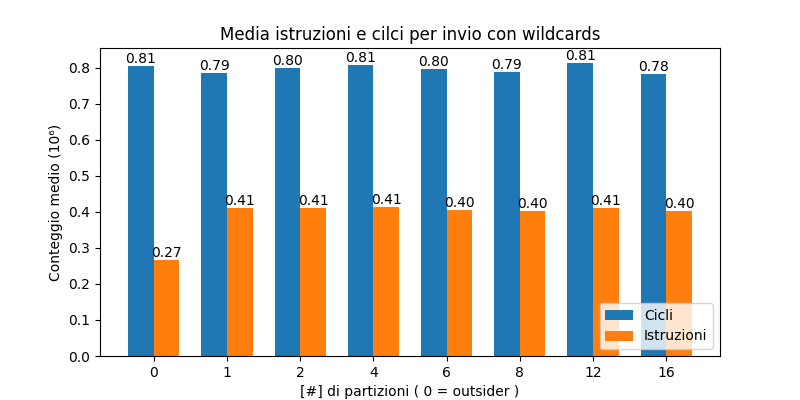
\includegraphics[width=\textwidth]{./results/test2_cyclinstr.png}
    \caption{Cicli e istruzioni necessari per invio con wildcards in diverse partizioni}\label{fig:test2cicl}
\end{figure}




\section{Throughput} % da sistemare test3 bandwidth, throughput e Freqeuncy
L'ultimo test, rivolto alla caratterizzazione della capacità di comunicazione, del middleware DDS, ci permette di capire il massimo scambio di dati che può avvenire tra i vari attori del Power Management. Nella figura \ref{fig:throughput_combined} l'asse Y, a sinistra, mostra in verde i il valore di KMessaggi/s~\footnote{1000 Messaggi al secondo} raggiungibili dai vari protocolli di comunicazione (in asse X), mentre in grigio, a destra i KByte/s. Dalla figura si può vedere che è possibile inviare ogni secondo da un publisher ad un subscriber più di un MB/s di dati. Inoltre è possibile raggiungere frequenze di scambio di messaggi dell'ordine di decine di KHz (\ref{fig:throughput_combined}). Inoltre, nel caso di invii a più subscriber, come si può vedere in figura~\ref{fig:bandwidth_graph}, mentre i protocolli udp shm tcp saturano all'aumentare del numero di subscriber, il protocollo UDP Multicast, permette una crescita lineare del throughput.

\begin{figure}[H]
    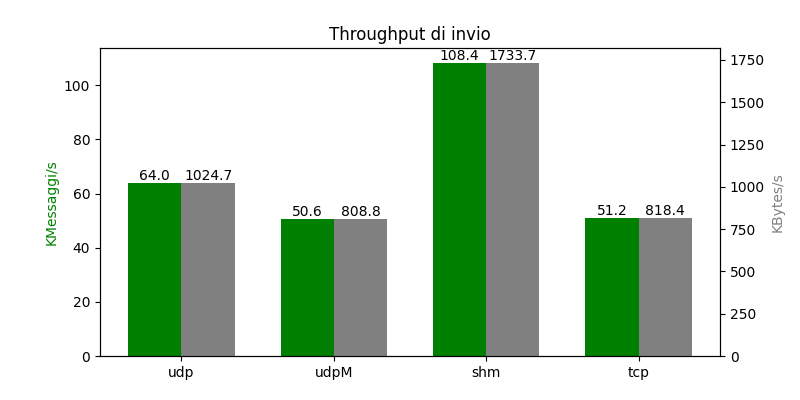
\includegraphics[width=\textwidth]{./results/test3_throughput_combined.png} 
        \caption{throughput con un publisher e un subscriber}\label{fig:throughput_combined}
\end{figure}

\begin{figure}[H]
    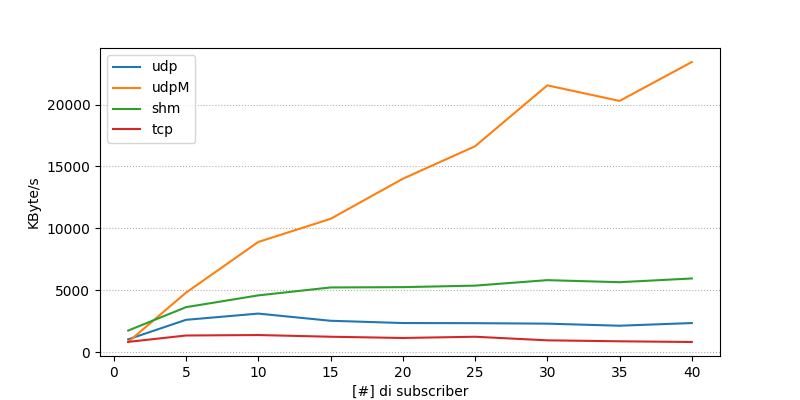
\includegraphics[width=\textwidth]{./results/test3_graph_throughput.png} 
    \caption{throughput a crescenti numeri di subscribers}\label{fig:throughput_increasing}
\end{figure}

Il risultato ottenuto nelle figure \ref{fig:throughput_combined} \ref{fig:throughput_increasing} (KBytes/s sulla Y e numero di subscriber sulla X), per quanto riguarda il protocollo UDP Multicast, è influenzato dalla struttura del test mostrato in figura \ref{fig:rtt_uml}, che non permette ad UDP Multicast di mostrare le sue potenzialita, come invece si può vedere dalla figura \ref{fig:bandwidth_graph}.

\begin{figure}[H]
    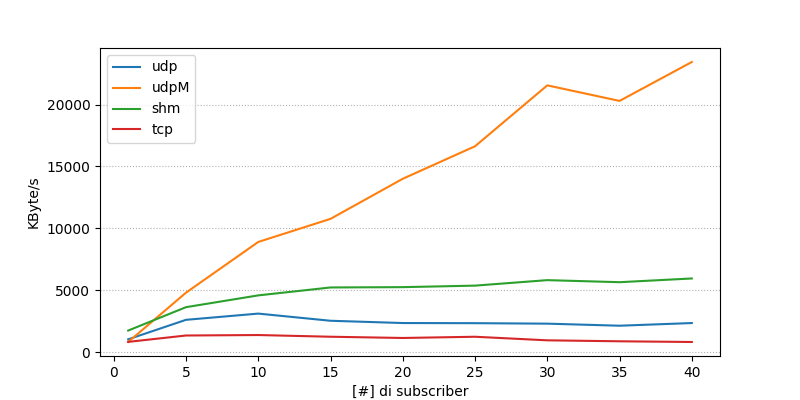
\includegraphics[width=\textwidth]{./results/test3_graph_bandwidth.png} 
        \caption{capacità di invio in KByte/s da un publisher a molteplici subscriber}\label{fig:bandwidth_graph}
\end{figure}

% Nella figura \ref{fig:bandwidth_combined} viene mostrato come un publisher usando multicast, viene liberato del suo incarico di inviare il messaggio ad ogni indirizzo di ogni subscriber, inviandolo ad un semplice indirizzo dove tutti i publisher riescono a 


\chapter{Realizzazione dei prototipi di Power Stack}
Nel corso di questa tesi con la collaborazione dei membri del progetto REGALE, come Cineca\cite{Cineca}, E4\cite{E4} e BSC\cite{BSC} sono stati sviluppati i middleware ed i prototipi di Power Stack per HPC. 
Questi ultimi oltre a fornire una prova della fattibilità nell'utilizzare una infrastruttura DDS come mezzo di comunicazione, sono utili anche come esempio per tutti quei software che devono essere introdotti nel progetto, mostrati nel capitolo~\ref{chap:4_REGALE}.
In merito a questo, nello schema~\ref{fig:schema_global_dummy_implementati} viene mostrato lo stato di avanzamento dei prototipi del Power Stack, illustrando quali di questi sono implementati e operativi, e quali in via di sviluppo.

\begin{figure}[H]
    \centering
    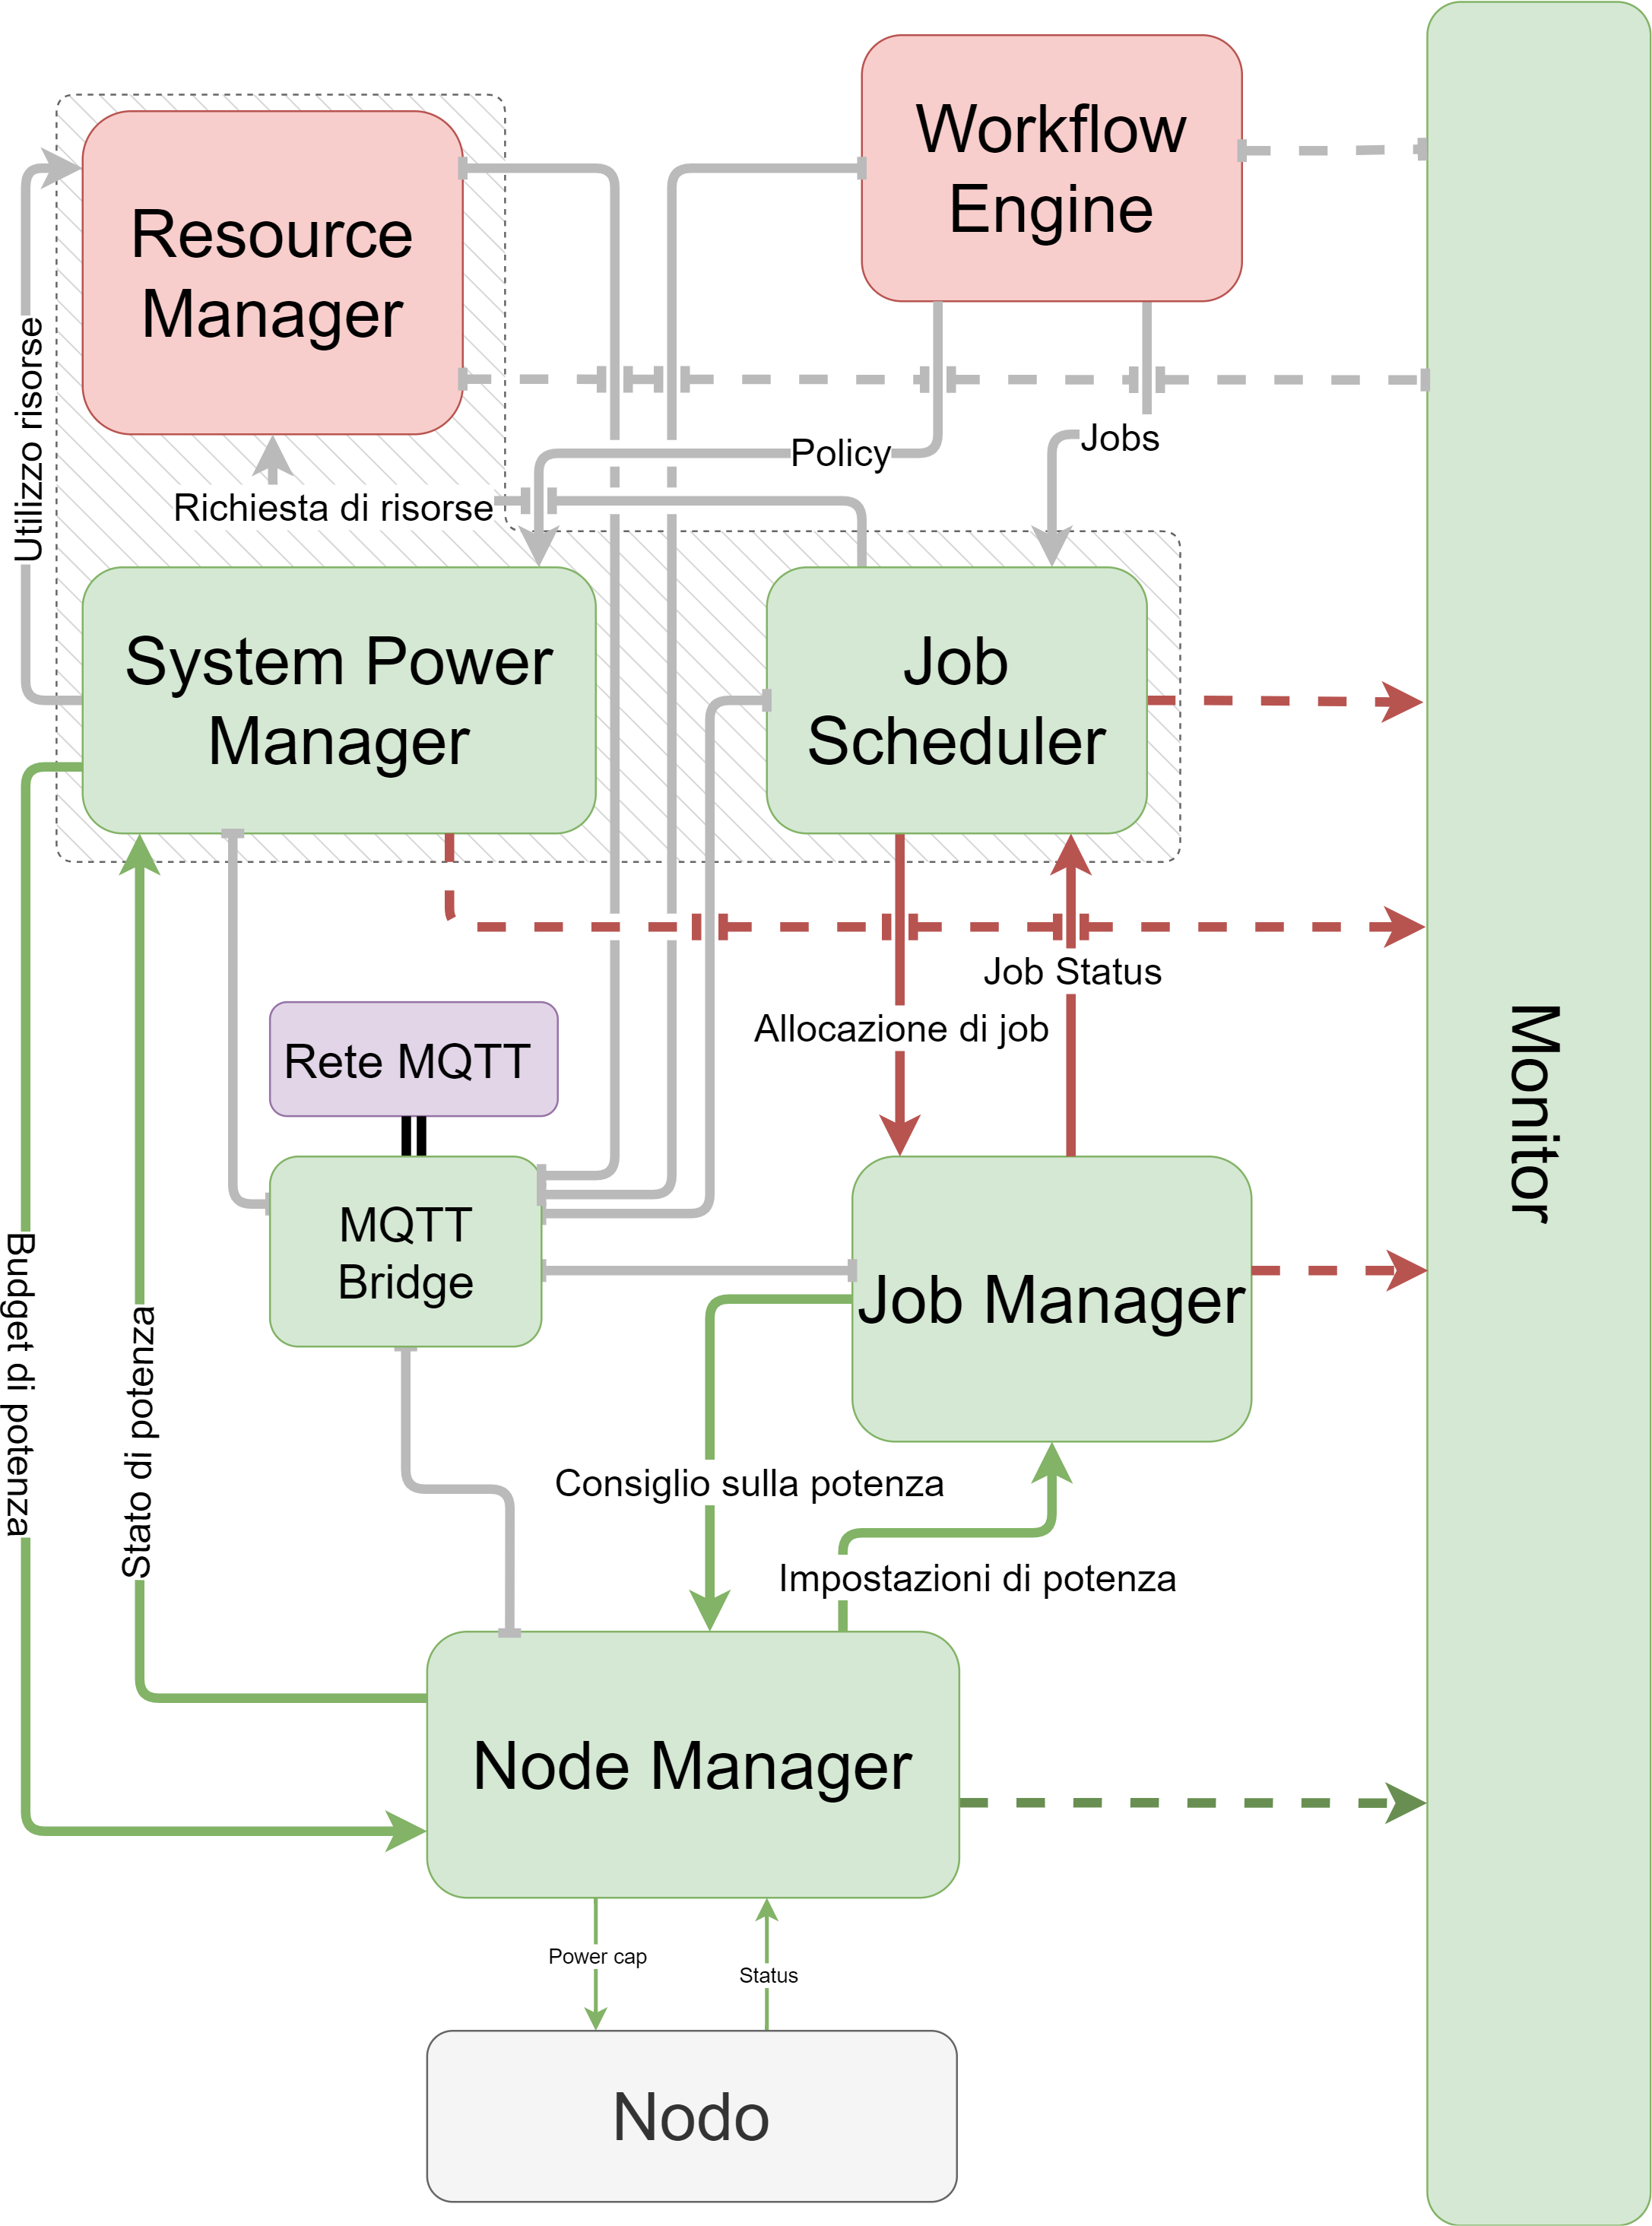
\includegraphics[width=0.50\textwidth]{./img/SchemaPowerStack_perdummy.drawio.png}
    \caption{Schema componenti sviluppati: in verde completato ed in rosso ancora da sviluppare}
    \label{fig:schema_global_dummy_implementati}
\end{figure}
L'infrastruttura DDS creata, chiamata \emph{REGALE Library}\cite{RegaleLibrary} al momento permette di utilizzare i vari tipi di comunicazione, configurazioni delle QoS, e anche vari tipi di dati scambiati, tutto impostabile tramite file \textbf{XML}.
I prototipi invece, sono dei programmi (c++) che vanno a simulare uno scambio di informazioni realistico. Al momento per motivi di semplicità utilizzano il protocollo \emph{UDP} e dati di tipo \emph{uint32\_t}. Il loro comportamento è riassumibile nel seguente modo.

\subsection*{Implementazione Job Scheduler}
Il JS interroga ogni 10 secondi il SPM per le informazioni sui servizi e la potenza totale del cluster riportandolo a schermo. Successivamente  imposta il limite di potenza del cluster con un valore casuale tra 1000 e 1500.

\subsection*{Implementazione Job Manager}
Il JM interroga il NM ogni 10 secondi e richiede il \emph{powercap} impostato e le informazioni sulle frequenze (massima, minima e corrente) riportando a schermo tutti i valori ottenuti.

\subsection*{Implementazione System power manager}
Il SPM nella sua implementazione server aspetta per le richieste in entrata. Al momento quelle previste sono:
\begin{itemize}
    \item GET\_INFO
    \item GET\_POWER
    \item SET\_POWER
\end{itemize}
%  ? Inoltre quando riceve una GET\_POWER il SPM inoltra la richiesta al NM per ottenere la sua potenza prima di rispondere alla richiesta. 

\subsection*{Implementazione Node manager}
Il NM mentre ogni 30 secondi manda i dati al Monitor, aspetta per le richieste in entrata. Le richieste accettate sono:
\begin{itemize}
    \item GET\_INFO\_NODE
    \item GET\_POWER\_NODE
    \item GET\_POWERCAP\_NODE 
    \item GET\_FREQ\_NODE   
    \item SET\_POWER\_NODE
\end{itemize}

\subsection*{Implementazione Monitor}
Il Monitor semplicemente aspetta che i componenti gli inviino i dati, e quando li riceve li riporta a schermo.

\subsection*{MQTT Bridge}
Questo componente, a differenza di tutti gli altri, non ha alcun ruolo nel Power Management ma serve solo a supporto di alcuni software che fanno ampio uso di comunicazioni MQTT\cite{mqtt}. Infatti, il suo scopo è quello di intercettare e convertire tutte le comunicazioni provenienti da MQTT e DDS per poi instradarle nel protocollo complementare.% Come dice il nome fa da \emph{ponte} tra le due infrastrutture, semplificando l'introduzione di alcuni software come Countdown\cite{cesarini2019countdown}.

\section{Struttura}
I componenti mostrati, al momento fanno uso delle strutture di domini, partizioni e topic mostrati in tabella~\ref{fig:dummy_topic}.

\begin{figure}[H]
    \centering
    \includegraphics[width=0.70\textwidth]{./img/server\_skeleton.png}
    \includegraphics[width=0.70\textwidth]{./img/dummies\_skeleton.png}
    \caption{Strutture di comunicazioni dei componenti implementati nel power stack.}
    \label{fig:dummy_topic}
\end{figure}
% In viola tutti i publisher, ed in giallo i subscriber. Successivamente nel rispettivo ordine vengono mostrati, domini, partizioni e topic utilizzati.

\chapter{Conclusioni}
Per concludere, dopo aver presentato in modo esaustivo tutti gli strumenti utilizzati per eseguire i test, con obbiettivi e metodi di sperimentazione, sono stati mostrati i risultati degli esperimenti fatti. 
In primo luogo si è visto l'andamento esponenziale nella fase di discovery, in presenza di molteplici partecipanti, risolvibile tramite la sua implementazione di server.
In secondo luogo, sono stati analizzati e caratterizzati i protocolli, tra cui il più performante si è rilevato essere quello di Shared Memory con una latenza media di ricezione messaggi di appena \SI{6.72}{\micro\second}, utilizzabile però solo in presenza di memorie condivise.
Al secondo posto troviamo UDP con \SI{23.7}{\micro\second} ed a seguire UDP Multicast con \SI{24.37}{\micro\second}, svantaggiato però dalla modalità utilizzata. Per ultimo TCP con \SI{30.94}{\micro\second} di media, che però offre garanzia di ricezione. Escludendo la shared memory, per le comunicazioni tramite rete si sono raggiunti throughput di 7.63 MB/s con frequenze di invio a 476 KHz.

Per quanto concerne al test sul partizionamento e sulle wildcards, si è visto come i domini sono quelli con minore impatto sulle performance, seguito dai topic ed infine partizioni. Inoltre, le minime differenze sia in termini di cicli, che di tempi, nell'usare le wildcards, permette un ampio uso di comunicazioni di tipo gerarchico.
Infine, insieme a questi risultati è stato fornito anche un modello di utilizzo di questo middleware in ambienti HPC.

Come ultimo passo, sono stati mostrati i middleware per la comunicazione basato su DDS, ed i prototipi di Power stack, entrambi prodotti in collaborazione con i membri del progetto EuroHPC JU REGALE.

%TODO: ringraziamenti? 

\printnoidxglossaries
\printbibliography

% \bibliography{references}

% \bibliographystyle{splncs04}
\end{document}
